\documentclass[a4paper,12pt]{book}
\usepackage{xcolor}
\usepackage{etoc}
\usepackage{soul}
\usepackage{blindtext}
\usepackage{scrextend}
\usepackage[utf8]{inputenc}
\usepackage[USenglish,british,american,australian,english]{babel}
\usepackage{helvet}
\usepackage{graphicx}
\usepackage{color}
\usepackage{geometry}
\usepackage{regexpatch,fancyvrb,xparse}
\usepackage{listings}
\usepackage{hyperref}
\usepackage{float}
\hypersetup{
    colorlinks,
    citecolor=black,
    filecolor=black,
    linkcolor=black,
    urlcolor=black
}
\lstset{
    frame=tb, % draw a frame at the top and bottom of the code block
    tabsize=4, % tab space width
    showstringspaces=false, % don't mark spaces in strings
    numbers=left, % display line numbers on the left
    commentstyle=\color{green}, % comment color
    keywordstyle=\color{blue}, % keyword color
    stringstyle=\color{red} % string color
}


\makeatletter
\let\do@footnotetext\@footnotetext
\regexpatchcmd{\do@footnotetext}
  {\c{insert}\c{footins}\cB.(.*)\cE.}
  {\1\c{egroup}}
  {}{}
\def\@footnotetext{\insert\footins\bgroup\@makeother\#\do@footnotetext}
\newcommand{\ttvar}{\begingroup\@makeother\#\@ttvar}
\newcommand{\@ttvar}[1]{\ttfamily\detokenize{#1}\endgroup}
\makeatother
\newcommand\tab[1][1cm]{\hspace*{#1}}
\geometry{hmargin={2cm, 2cm}, height=10.0in}

\begin{document}
\thispagestyle{empty}
%% ------------------------ NAGLOWEK STRONY ---------------------------------

\includegraphics[height=37.5mm]{agh_nzw_a_en_1w_wbr_pms}\\
\rule{30mm}{0pt}{
{\large \textsf{Faculty of Physics and Applied Computer Science}}\\
\rule{\textwidth}{3pt}\\
\rule[2ex]
{\textwidth}{1pt}\\
\vspace{7ex}
\begin{center}
{\LARGE \bf \textsf{Engineering thesis}}\\
\vspace{13ex}
% --------------------------- IMIE I NAZWISKO -------------------------------
{\bf \Large \textsf{Michal Stefaniuk}}\\
\vspace{3ex}
{\small \sf major: {\bf \textsf{applied computer science}}}\\
\vspace{1.5ex}
%{\small \sf specialisation: {\bf \textsf{software engineering}}}\\
\vspace{10ex}
%% ------------------------ TYTUL PRACY --------------------------------------
{\bf \huge \textsf{Web application developement using WebToolkit
C++ on the example of a banking service}}\\
\vspace{14ex}
%% ------------------------ OPIEKUN PRACY ------------------------------------
{\Large \sf Supervisor: {\bf \textsf{Dr Grzegorz Gach}}}\\
\vspace{22ex}
{\large \bf \textsf{Cracow, Januray 2021}}
\end{center}
%% =====  STRONA TYTULOWA PRACY MAGISTERSKIEJKIEJ ====

\newpage

\begin{center}
	{\bf\large\textsf{Oświadczenie studenta}}\\
\end{center}

%% ===== PL TYL STRONY TYTULOWEJ PRACY MAGISTERSKIEJKIEJ ====
{Uprzedzony(-a) o odpowiedzialnosci karnej na podstawie art. 115 ust. 1 i 2 ustawy z dnia 4 lutego 1994 r. o prawie autorskim i prawach pokrewnych (t.j. Dz. U. z 2018 r. poz. 1191 z pozn. zm.): ,,Kto przywlaszcza sobie autorstwo albo wprowadza w blad co do autorstwa calosci lub czesci cudzego utworu albo artystycznego wykonania, podlega grzywnie, karze ograniczenia wolnosci albo pozbawienia wolnosci do lat 3. Tej samej karze podlega, kto rozpowszechnia bez podania nazwiska lub pseudonimu tworcy cudzy utwor w wersji oryginalnej albo w postaci opracowania, artystyczne wykonanie albo publicznie znieksztalca taki utwor, artystyczne wykonanie, fonogram, wideogram lub nadanie.", a takze uprzedzony(-a) o odpowiedzialnosci dyscyplinarnej na podstawie art. 307 ust. 1 ustawy z dnia 20 lipca 2018r. Prawo o szkolnictwie wyzszym i nauce (Dz. U. z 2018 r. poz. 1668 z pozn. zm.) ,,Student podlega odpowiedzialnosci dyscyplinarnej za naruszenie przepisow obowiazujacych w uczelni oraz za czyn uchybiajacy godnosci studenta.", oswiadczam, ze niniejsza prace dyplomowa wykonalem(-am) osobiscie i samodzielnie i nie korzystalem(-am) ze zrodel innych niz wymienione w pracy.

\bigskip

Jednoczesnie Uczelnia informuje, ze zgodnie z art. 15a ww. ustawy o prawie autorskim i prawach pokrewnych Uczelni przysluguje pierwszenstwo w opublikowaniu pracy dyplomowej studenta. Jezeli Uczelnia nie opublikowala pracy dyplomowej w terminie 6 miesiecy od dnia jej obrony, autor moze ja opublikowac, chyba ze praca jest czescia utworu zbiorowego. Ponadto Uczelnia jako podmiot, o ktorym mowa w art. 7 ust. 1 pkt 1 ustawy z dnia 20 lipca 2018 r. Prawo o szkolnictwie wyzszym i nauce (Dz. U. z 2018 r. poz. 1668 z po 'zn. zm.), moze korzystac bez wynagrodzenia i bez koniecznosci uzyskania zgody autora z utworu stworzonego przez studenta w wyniku wykonywania obowiazkow zwiazanych z odbywaniem studiow, udostepniac utwor ministrowi wlasciwemu do spraw szkolnictwa wyzszego i nauki oraz korzystac z utworow znajdujacych sie w prowadzonych przez niego bazach danych, w celu sprawdzania z wykorzystaniem systemu antyplagiatowego. Minister wlasciwy do spraw szkolnictwa wyzszego i nauki moze korzystac z prac dyplomowych znajdujacych sie w prowadzonych przez niego bazach danych w zakresie niezbednym do zapewnienia prawidlowego utrzymania i rozwoju tych baz oraz wspolpracujacych z nimi systemow informatycznych.}\\

\newpage
\begin{flushleft}
{\bf\large\textsf{Streszczenie pracy}}\\
\end{flushleft}
{
\tab Celem niniejszej pracy dyplomowej bylo zaimplementowanie aplikacji pozwalajacej wykorzystac w procesie tworzenia rozmaite narzedzia programistyczne. Narzedzia, o ktorych mowa to przede wszystkim programy wspomagajace inżnynierie oprogramowania i sa one wykorzystywane w dzisiejszych czasach przez wielu programistow. 

\bigskip
Tematem programu jest internetowa aplikacja bankowa umozliwiajaca trywialne funkcjonalnosci takiego serwisu, jak na przyklad przelewanie pieniedzy czy przegladanie logow transakcyjnych przez administratora. Calosc zostala zaimplementowana w jezyku C++ ze wsparciem biblioteki WebToolkit. Narzedzia, ktore wykorzystano do wspomozenia procesu inzynierii oprogramowania to system kontroli wersji GitHub, automatyczny serwer regresyjny GitHub oraz oprogramowanie do sledzenia postepow i zarzadzania projektami JIRA.
}

\bigskip
\begin{flushleft}
{\bf\large\textsf{Abstract}}\\
\end{flushleft}
{
\tab The goal of this thesis was implementing an application that would allow to use various  software engineering tools during the development process. Those tools are especially the ones that are enhancing the process and nowadays they are used by almost every programmer.

\bigskip
The topic of the program is a web application as a banking service that provides simple features like wiring money or going through service logs to the users and admin. The code was written in C++ language with support of Web Toolkit library. The tools used in this project to conduct the software engineering processes were version control system GitHub, autmatic regression GitHub server and issue tracking tool JIRA. 
}
	

\tableofcontents
\chapter*{Introduction}
\addcontentsline{toc}{section}{\protect\numberline{}Introduction}%
\tab {Software engineering is a very wide area of engineering which particularly concerns developing and maintaining programming products. A development process itself is a major challenge to all people involved, starting with engineers creating the code, continuing with product owners who are managing teams and coordinating the work flow and ending-up with managers who are setting the direction of the whole process.

\bigskip
The main motivation to create this thesis was simply to present a development process that includes basic and nowadays necessary tools which are significantly helpful in such process. Simultaneously creating a C++ web application was an equally important factor. To carry out the development and present all tools it was decided that an example C++ web application will be created with a GUI library in modern C++ called \textbf{Web Toolkit}. 

\bigskip 
Nowadays in a software engineering world there is a trend to migrate desktop applications to the internet, which has also impacted a lot GUI desktop libraries in decreasing their utilities. The secondary reason behind choosing C++ to create a web application, which is quite unusual, was to show the tremendous possibilities that this language still provides and to exhibit the capabilities of open source libraries shared among developers and engineers. The bottom line is - next chapters are a review of possibilities that C++-based web library provides.
}

\chapter{Projects assumptions}

\section{Application's blue-print}
{
The application is a single-page service run on a local server with an \textbf{http://localhost:8080/} address. After starting, logging panel appears, giving the user an opportunity to type their credentials and log-in. 

\bigskip
The idea of the service is to provide basic functionalities of a banking service like for instance transferring money or checking their balance to the user. These required implementation of secure back-end layer with a database containing information about the users and transactions and a front-end layer which is transparent to the user. 

\bigskip
Regarding the credentials a user will see different features after logging into the service. There might be many accounts created and held up in the database of the service but there are only two rights of access.}\\
\begin{labeling}{alligator}
\item [\textbf{USER}] Transferring money and seeing current account's balance.
\item [\textbf{ADMIN}] Seeing details about every account in the service as well as having access to the logs from the application.
\end{labeling}

\bigskip
After user decides to quit the service, a possibility of logging out is provided and whilst doing that the application returns to the logging page where session is refreshed and database is updated. If the user was an administrator of the service, an access to the console logs that are gathering and sniffing network traffic like HTTP methods for RESTful APIs is also granted.  

\section{Programming environment}
{\tab Developing any kind of programs usually requires specific environmental variables therefore a programmer's task is to choose a specific set of tools which will be the most handy during the process.  

\bigskip
Regarding the specifics of the project, the chosen set of tools looks like following:
\begin{labeling}{alligator}
\item [\textbf{IDE}] Microsoft Visual Studio Community 2019,
\item [\textbf{LIBRARY}] Web Toolkit 4.3.1,
\item [\textbf{LIBRARY}] Boost C++ lib [latest version],
\item [\textbf{TOOL}] CMake VERSION 2.4,
\item [\textbf{TOOL}] Git BASH.
\end{labeling}}

The application was developed under Windows 10 64-bit operating system, but it could have been developed under any other platform that is supported by WebToolkit library.

\newpage
\subsection*{IDE - Integrated Development Environment}
{
\tab IDE is a program or a set of programs merged into one that usually gathers tools, libraries, debuggers, run time scripts and any other stuff necessary for the developer to write the code. The purpose of IDE is to allow easily and swiftly create code, but at the same time test it, compile it and run it in one place. 

\bigskip
The advantage of this solution is that it gives the developer an opportunity to set up and scale his development environment adjusting it to the project needs. Usually IDE, as well as modern text editors, also support plugins which are nice addition to the program, like for instance syntax highlighters, semantics hints, code analyzers or refactoring scripts.

\bigskip
The chosen IDE for this project is \textbf{Microsoft Visual Studio Community 2019}. Web Toolkit library is supported on various platforms including Linux distributions (even less popular ones like ArchLinux, Slackware or Opensuse), Windows or other operating systems like Android, Raspberry Pi or even OS X. The consequence of choosing MSV IDE was using Windows platform and prebuilt Windows binaries of the WT library.

\bigskip
\textbf{Microsoft Visual Studio} is an IDE produced by Microsoft Company and it allows creating cross-platform software with graphical user interface. It basically supports every programming language but the basic package contains support for 
\begin{itemize}
	\item Microsoft Visual C,\ttvar{#}
	\item Microsoft Visual C++,
	\item Microsoft Visual Basic,
	\item Microsoft Visual J,\ttvar{#}
	\item Microsoft Visual Web Developer ASP.NET,
	\item Microsoft Visual F.\ttvar{#}
\end{itemize}

Microsoft Visual Studio (MSVC) also provides a lot of built-in features. Many of them occurred to be significantly useful in the process of developing this application. A few most important ones are
\begin{itemize}
	\item debugger, linker and compiler,
	\item projects and build systems,
	\item writing and refactoring C++ code,
	\item code analysis overview,
	\item unit tests support,
	\item universal windows apps like command line appliactions.
\end{itemize}

}

\subsubsection*{Boost C++ library}
{
\tab Boost is a collection of C++ libraries that enhances capabilities of C++ code development, which is also licensed by \textbf{Boost Software License}. For the project Boost is necessary to build Web Toolkit library as it's implementation uses Boost functionalities.

\bigskip
The most important features provided by Boost are
\begin{itemize}
	\item algorithms,
	\item concurrent programming,
	\item complex containers,
	\item correctness validating and enhanced unit testing,
	\item additional data structures (like bimap, fusion, tuple etc),
	\item high level programming and functional objects,
	\item parsers and graphs,
	\item meta-programming with templates.
\end{itemize}
	
Boost library as a collection is not used in this project explicitly, as the application was developed in Microsoft Visual Studio environment with pre-built Windows binaries. However, for automation server, the project is built with linux machine where WebToolkit needs to be built manually, therefore boost is required.
}
\subsubsection*{CMake}
{
\tab CMake is a cross platform tool that provides automatic management of compiler that builds the code of an application. It's role is to create a configuration for project files of popular programming environments, which then are used in a process of compilation. The main advantage of using CMake is it's independence of the compiler and the platform. Moreover CMake as a standalone program creates files with rules for compilation dedicated to another program like IDE and it forms a unified building environment. CMake stands for \textit{Cross-platform Make}.

\bigskip
The most important features provided by CMake are
\begin{itemize}
	\item platform independence,
	\item cross compilation,
	\item out-of-source building,
	\item building projects with complex catalog structure,
	\item unit testing support,
	\item detecting dependencies and outer libraries.
\end{itemize}
This project required including CMake tool because of various dependencies and complex building due to including Web Toolkit and Boost.  

\bigskip
To be able to explore favors that CMake offers one must create \textbf{CMakeLists.txt} file placed in the desired catalog of the project. The core of this file is a simple scripting language that describes rules and defines variables telling the compiler how to link files and what should be the outcome of the compilation process.

\bigskip
Let's have an example project\cite{cmakeintroduction} which structure looks like below.\newline
\begin{lstlisting}[frame=single, language=C++, caption={Example CMake project structure.}, captionpos=b]
 .
 |-- CMakeLists.txt
 |-- build
 |-- include
 |   \-- Student.h
 \-- src
     |-- Student.cpp
     \-- mainapp.cpp
\end{lstlisting}

\bigskip
The content of \textbf{*.cpp} and \textbf{*.h} files is irrelevant here, at this point it could be any code. In the main directory there is a simple \textbf{CMakeLists.txt} which is used to build the project. The code of the \textbf{CMakeLists} script:\newline

\begin{lstlisting}[frame=single, language=C++, caption={CMakeLists.txt of example project.}, captionpos=b]
cmake_minimum_required(VERSION 2.8.9)
project(directory_test)

#Specifies include directories to use when compiling a given target
include_directories(include)

#Can manually add the sources using the set command as follows:
#set(SOURCES src/mainapp.cpp src/Student.cpp)

#However, the file(GLOB...) allows for wildcard additions:
file(GLOB SOURCES "src/*.cpp")

add_executable(testStudent ${SOURCES})
\end{lstlisting}
\bigskip
The most important things while building the project that above CMake will perform (in order from the top) are
\begin{itemize}
	\item Include directories to specify headers files directories
	\item Sources are also set, but the line is commented out as each file needs to be manually added in place
	\item file() command to add source files to project's GLOB SOURCES
	\item add\_executable() which uses SOURCES variable in order to build executable program
\end{itemize}


\noindent Now to invoke building using CMake:
\begin{lstlisting}[language=bash]
  $ cd build
  $ cmake ..
  $ make
  $ ./testStudent
\end{lstlisting}
  
\bigskip First current directory is changed to build, where output files will be stored. From there cmake will create \textbf{Makefile} containing references to all sources and headers, which ultimately will create an executable that is ready to be run. This as a very basic example of how \textbf{CMake} works. In next chapters there will be more details about \textbf{CMake} and what is the main concept behind basing on the one used in project. 

}

\chapter{WebToolkit C++ library}
\section{Library overview}
{\tab \textbf{Web Toolkit} is an open-source C++ library that allows developers to create Single Page web applications without writing single line of JavaScript code. The main concept behind SAP~\cite{singlepageapplications}(\hl{Single Page Applications}) is they do not render HTML files, but instead they use asynchronous JavaScript to reload contents of the page in real time without refreshing the whole page. To some extent it might be a bit misleading, as with loading different content, the URL of the page changes as well, like in ordinary multi-page service.

\begin{figure}[h]
  \centering
    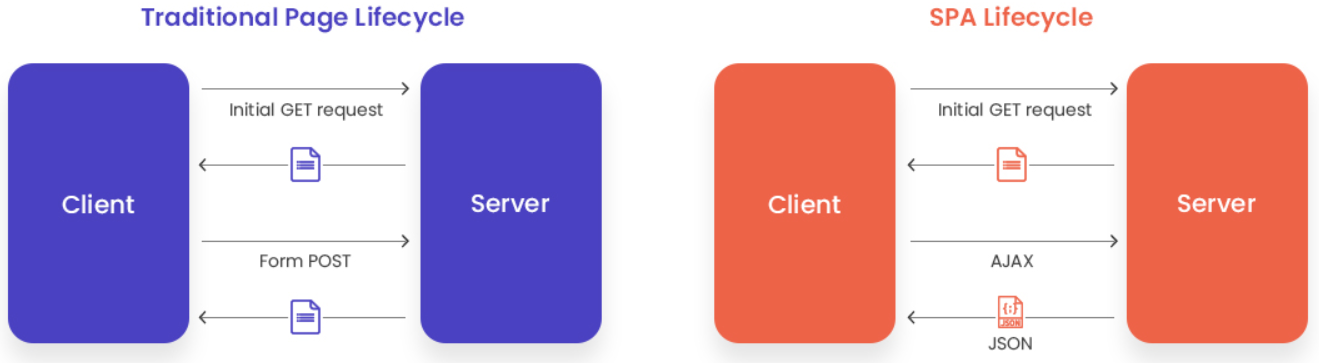
\includegraphics[width=1.0\textwidth]{spa}
    \caption{Traditional Page vs SPA.}
\end{figure}

\bigskip
As a SPA, web-banking application works on widgets which are the core of WebToolkit library. A widget itself is a specific type of user-computer interaction with a graphical interface such as button or a scroll bar, which in WebToolkit case is wrapped in C++ code. A developer should create a main widget, which is not visible to the user. Instead it works as a widget container that will hold other template widgets that will be plugged in or plugged out depending on what content will be loaded on the page.  

\begin{figure}[h!]
\centering
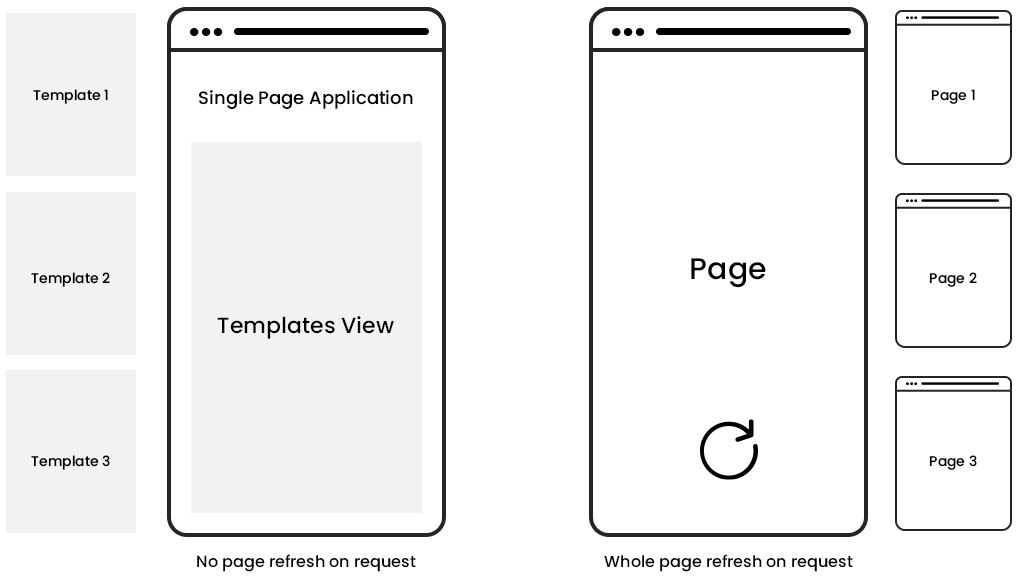
\includegraphics[width=1.0\textwidth]{spa-template}
\caption{Views in Traditional Page and SPA[2].}
\end{figure} 

\bigskip
There are a lot of modern services that use SPA technology like facebook~\cite{facebook}, airbnb~\cite{airbnb}, twitter~\cite{twitter}, paypal~\cite{paypal}, gmail~\cite{gmail} or even netflix~\cite{netflix}. The biggest benefits of this web application model are quick loading time, good caching abilities, improved user experiance or rapid front-end development. 

\bigskip
The most important thing about Single Page Application model is very rapid and fast user experience as the page does not refresh or re-render. However, since the page works on widgets usually the HTML contents of the page is rather empty. Often it's just a few tags, scripts and imports while the rest of the contents is loaded dynamically for instance by asynchronous javascript. This is a big disadvantage when it comes to search engines that are using crawlers. Instead of seeing the web contents they will see a short HTML file with not too much to process, since crawlers never wait for asynchronously loaded data. This SEO problem makes Single Page applications a bad choice for services relying on search engines and positioning.

\bigskip
On the other hand a regular static page has a lot to offer too. It servers HTML file instantly, but it requires refreshing and rendering new page. It reduces the amount of javascript code that is needed but it also allows crawlers to see the same content that users can see. The disadvantage of this type of page should be pretty obvious now - it allows to create services with limited dynamic content. It might be a poor choice to go for when a service needs to serve content that changes quite frequently.


\bigskip
Beyond usual frameworks dedicated for SPA services are
\begin{itemize}
	\item Angular.js,
	\item React.js,
	\item Backbone.js,
	\item Ember.js.
\end{itemize}

It is no secret that preferable programming technology stack for such development would be JavaScript~\cite{javascript}, TypeScript~\cite{typescript}, HTML~\cite{html}, CSS~\cite{css} and some back-end in Java~\cite{java}, Python~\cite{python} or PHP~\cite{php}. With that being said, WebToolkit library seems to be very unorthodox tool for this task. The whole development process starts and ends with C++ code, which makes it interesting and unusual.

\newpage

}
\section{WebToolkit Features}
{
\tab \textbf{Web Toolkit} library has a lot to offer. Now of course - creating web application in C++ language comes with a prize. It's biggest disadvantage is that while programming we have no control of HTML code. There is also a necessity of re-compiling the code with every change introduced where there is no such need when using standard web development tools (like javascript application with node.js or php application with XAMPP). However, having said that it is worth mentioning that Web Toolkit is appreciated for plenty features that it provides to the users.
 
\begin{figure}[h]
  \centering
    
\includegraphics[width=0.7\textwidth]{features}
    \caption{WebToolkit logo and features~\cite{wtlogo}.}
\end{figure}

\subsection*{Core Library} 
{
\tab What is really important is that core library is fully open source and still under development. It's implementation allows to integrate it with third party JavaScript libraries, which is a nice addition for developers that create services with more advanced front-end layer. What is more, Web Toolkit is fully compatible with HTML5~\cite{html5} and HTML4~\cite{html4} browsers. Thus, as a hybrid single page framework it supports browser history navigation. The bottom line is, WT is a high performance library which is something you would expect from a C++ library. It is optimized when it comes to asynchronous I/O, multi-threading and throughout all rendering.

\bigskip
Event handling is completed with C++11 lambdas~\cite{lambda} or bound object methods to retreive data that is bound to a function. Those are a part of C++11 signal/slot API for responding to various events. Server-initiated updates are also available through WebSockets and automatic fallaback to AJAX. Event handling itself is also completed with efficient synchronization of browser using session, which incrementally renders updates of application states.

\bigskip
Core library also provides 2D and 3D painting support to users and developers. Through Web Toolkit API it is possible to generate simple graphics objects like HTML5 canvas, inline SVG~\cite{svg} or inline VML. Graphics is also leveraged by rendering common image formats like PNG, GIF or even PDF. WT broads the variety of graphics support by also supporting hardware-accelerated 3D painting API like for instance server-side OpenGL~\cite{opengl}.
}

\subsection*{Security}
{
\tab As a completed web-development library, WebToolkit provides built-in security layer to the applications which contains:

\begin{itemize}
	\item kernel-level memory protection in isolated sessions,
	\item TLS/SSL support,
	\item Cross-Site Scripting (XSS) prevention,
	\item Request Forgery (CSRF) prevention,
	\item Application logic attack prevention,
	\item DoS mitigation,
	\item \textbf{Authentication module} (including support for OAuth 2.0 and OpenID Connect).
\end{itemize}

\begin{figure}[h]
  \centering
    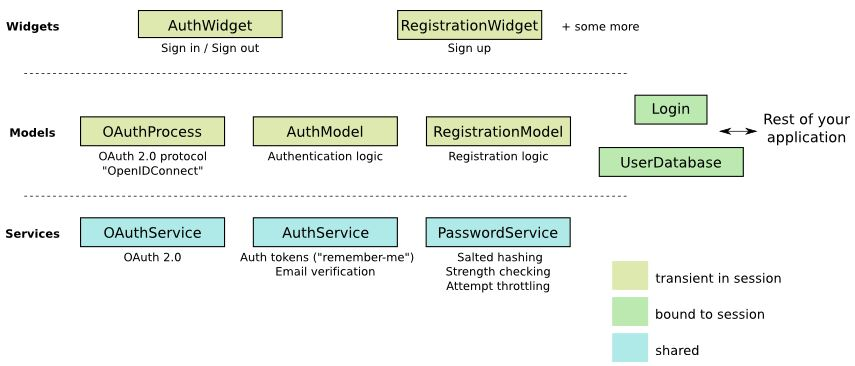
\includegraphics[width=1.1\textwidth]{auth-module}
    \caption{Main classes of the authentication module\cite{authmodule}.}
\end{figure}

The authentication module itself occurred to be significantly important and helpful in Web Banking Application. Some of the classes which implement basic user features are presented above. What it means is that secure and robust service functionalities like signing in/out, registration or authentication are already provided.

}

\subsection*{Database support}
{
\tab As any other modern library, WT supports databases with a sub-library called Wt::Dbo, which by implementing ORM (Object-Relational Mapper) becomes a convenient way to communicate C++ application with SQL databases. What is more, Wt::Dbo as a self-contained sub-library is independent from Wt itself, which means it could be used for standalone back-end service. Other basic Wt::Dbo features are: 

\begin{itemize}
	\item Support for
	\begin{itemize}
     \item Sqlite3
     \item Firebird
     \item MariaDB
     \item MySQL
     \item SQL Server
     \item PostgreSQL
     \end{itemize}
	\item Native SQL to query objects and fields
	\item Session with first-level cache
	\item DB transactions
	\item CRUD operations
	\item Many-to-One and Many-to-Many relations
	\item Just C++ without XMLs or Macros

\end{itemize}
}

\subsection*{Deployment}
{
\tab Extremely important thing in any application is process of Deployment. WT through various abstract interfaces connects with outer world. The basic one is built-in httpd but among others:

\begin{itemize}
	\item Built-in \textbf{HTTPD}
	\begin{itemize}
     \item Simple and high performance with multithreading and asynchronous I/O based on C++ asio library
     \item Supports WebSockets and HTTP(s) with chunking and compression
     \item Available for many platforms like Linux, Windows and any UNIX like systems
     \end{itemize}
	\item \textbf{FASTCGI}
	\begin{itemize}
     \item Integrated with common web servers like apache
     \item Supported for Linux and UNIX
     \end{itemize}
	\item \textbf{ISAPI}
	\begin{itemize}
     \item Integrated with Microsoft IIS server
     \item Completed with asynchronous API
     \item Supported for Windows
     \end{itemize}
\end{itemize}
}
\newpage
}

\section{Hello World Application}
{
Lets go through simple Hello World applications just to get in touch with WebToolkit library environment.

\begin{lstlisting}[frame=single, basicstyle=\small, language=C++, caption={A complete "Hello world" application \cite{helloworldapp}.}, captionpos=b]
#include <Wt/WBreak.h>
#include <Wt/WContainerWidget.h>
#include <Wt/WLineEdit.h>
#include <Wt/WPushButton.h>
#include <Wt/WText.h>

class HelloApplication : public Wt::WApplication
{
public:
    HelloApplication(const Wt::WEnvironment& env);

private:
    Wt::WLineEdit *nameEdit_;
    Wt::WText *greeting_;
};

HelloApplication::HelloApplication(const Wt::WEnvironment& env)
    : Wt::WApplication(env)
{
    setTitle("Hello world");

    root()->addWidget(std::make_unique<Wt::WText>("Your name, please? "));
    nameEdit_ = root()->addWidget(std::make_unique<Wt::WLineEdit>());
    
    Wt::WPushButton *button = 
    	root()->addWidget(std::make_unique<Wt::WPushButton>("Greet me."));
    	
    root()->addWidget(std::make_unique<Wt::WBreak>());
    greeting_ = root()->addWidget(std::make_unique<Wt::WText>());
    
    auto greet = [this]{
      greeting_->setText("Hello there, " + nameEdit_->text());
    };
    button->clicked().connect(greet);
}

int main(int argc, char **argv)
{
    return Wt::WRun(argc, argv, [](const Wt::WEnvironment& env) {
      return std::make_unique<HelloApplication>(env);
    });
}
\end{lstlisting}

\newpage
Now when it comes to building, it could be done locally by setting up a localhost HTTP server. Having IDE set-up it is done automatically. Otherwise while operating on UNIX-like systems:

\begin{lstlisting}[frame=single, basicstyle=\small, language=C++, caption={Building "Hello world" application.}, captionpos=b]
$ g++ -std=c++14 -o hello hello.cc -lwthttp -lwt
$ ./hello --docroot . --http-address 0.0.0.0 --http-port 9090
\end{lstlisting}

\bigskip
The final result is:
\begin{figure}[h]
  \centering
    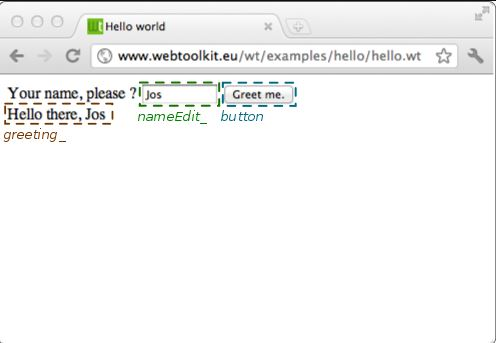
\includegraphics[width=0.7\textwidth]{hello-app}
    \caption{Hello Application on Web Toolkit.}
\end{figure}

\bigskip
The above code presents basic concepts of the library workflow.

\begin{labeling}{alligator}
\item [\textbf{class HelloApplication}] A class that represents application and extends Wt::WApplication. Contains ctor that takes Wt::WEnvironment and private fields that represents input field and output greeting string wrapped in Wt::WText.
\item [\textbf{LINE 20:}] Sets title of appliaction which will be visible in web browser's card.
\item [\textbf{LINE 22-29:}] This part of the code handles adding widgets to the root which represents a container for the widgets. This is an implementation of SPA concept where we create widgets and plug them in or out, for instance by addWidget() function.
\item [\textbf{LINE 31:}] Lambda expression that returns WText string which is called upon clicking the button.
\item [\textbf{LINE 34:}] Calling lambda expression from line 31 when button is clicked.
\item [\textbf{MAIN:}] Creating and running application.
\end{labeling} 


}
\section{Widgets gallery}
{
\tab \textbf{Web Toolkit} also offers a widgets gallery, which is nothing else but a bootstrap where most common widgets are already implemented and ready to be used. Among them there are layouts, forms widgets, navigation widgets, trees widgets, tables widgets, graphics widgets, charts widgets and media widgets. Basically whilst going through development process one should keep in mind this feature as it may save a lot of time and a lot of coding. 

\bigskip
\begin{figure}[h]
  \centering
    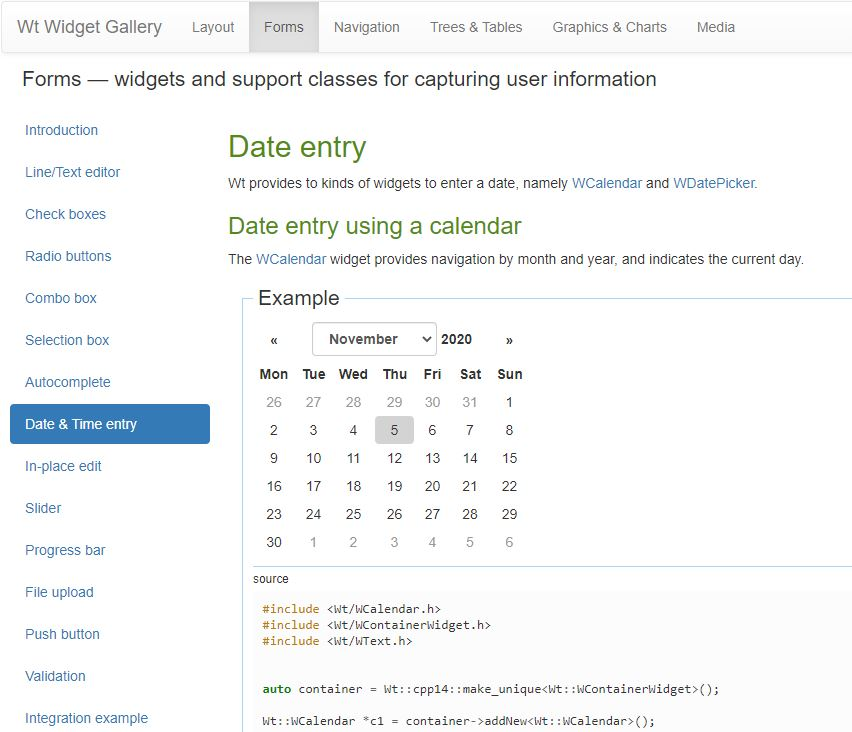
\includegraphics[width=1.0\textwidth]{gallery}
    \caption{Web Toolkit Widget Gallery.~\cite{widgetsgallery}.}
\end{figure}
    
     
}

\chapter{DevOps layer}
\section{Introduction}
{
\tab DevOps stands for development and operations and it is a modern approach for software engineering. Its core is to integrate developer teams with other sections invloved in the process. According to this definition, DevOps engineer is someone who is fluent with development cycle and it is also someone who can improve the process. Naturally there are a lot of cutting-edge tools which are significantly helpful in DevOps engineering. 

\bigskip
\begin{figure}[H]
  \centering
    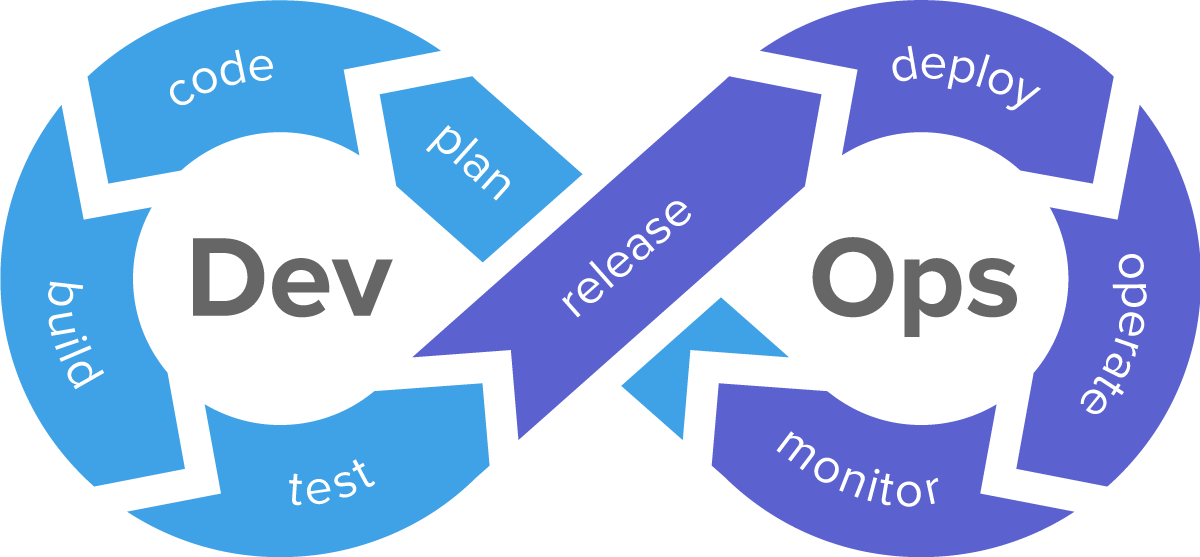
\includegraphics[width=0.8\textwidth]{devops}
    \caption{DevOps process.~\cite{devops}.}
\end{figure}
    
Figure 3.1 shows basic elements of devOps approach which are
\begin{itemize}
	\item building the product that is being developed,
	\item coding,
	\item planning the whole process,
	\item monitoring the development,
	\item operating,
	\item deploying for instance to cloud,
	\item releasing to client,
	\item and testing throughout the whole time.
\end{itemize} 
	
\bigskip
Creating web banking application was also about carrying out the development process based on DevOps approach. 
}
\section{Distributed version-control system}}
{
\tab First tool that was used in this project was version-control system called \textbf{Git}. It is a tool that allows developers to track changes in code of the project, as well as making them. Every change introduces a new version of the code which is stored in history. The biggest advantage of this feature is capability of restoring previous version of the code which presents tremendous enhancement to reponsing to unwanted changes.

\bigskip
What is more, Git provides branching feature, which simplifies developing code simultaneously by many developers at the same time. By invoking simple command line functions developer can communicate his local repository with remote repository. Many version-control systems have graphic interfaces too.

\bigskip
\begin{figure}[H]
  \centering
    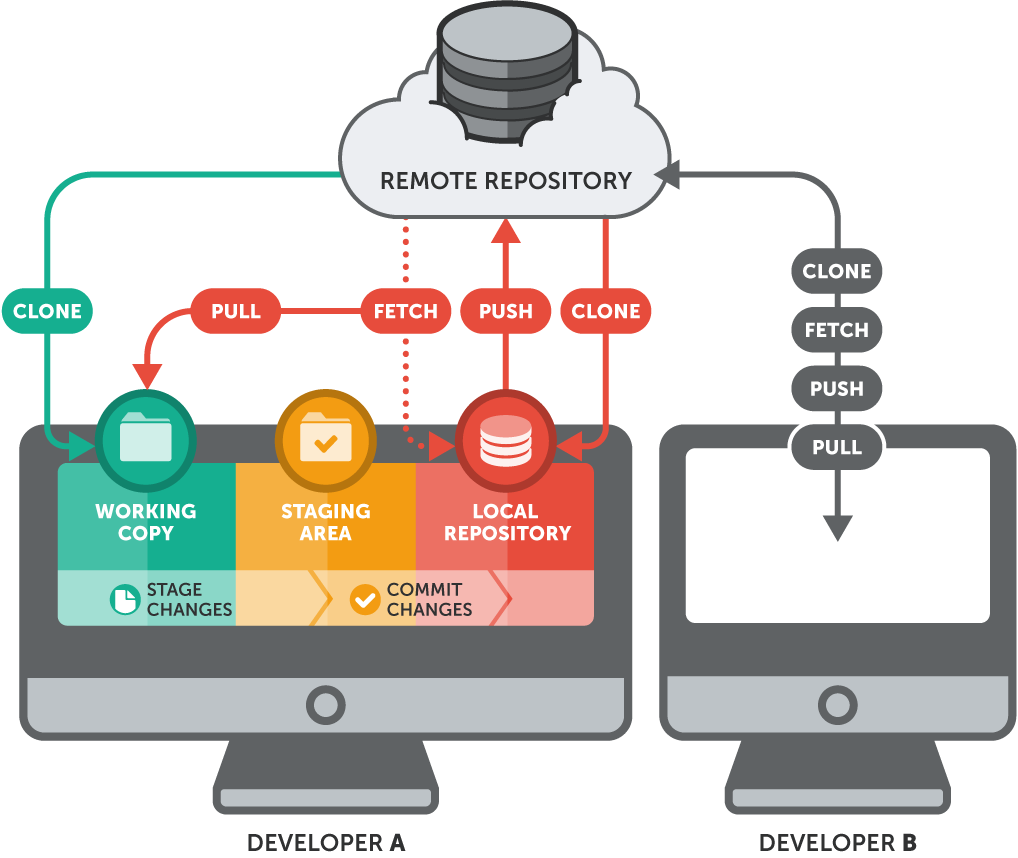
\includegraphics[width=1.0\textwidth]{git}
    \caption{Distributed version-control system workflow.~\cite{git}}
\end{figure}   
}
\section{GitHub}
{
\tab Web banking application was being developed using GitHub, which is a GIT version-control system hosting dedicated for programming projects. A remote repository was stored there, which contained:

\begin{itemize}
	\item applications code,
	\item CMake building scripts,
	\item YAML docker images for automation server,
	\item web toolkit library,
	\item static resources like images,
	\item unit and regression tests,
	\item this theesis,
	\item and most importantly - information about all changes introduced to the project.
\end{itemize}
	
\bigskip
Creating this application required over 150 commits, 18 branches and more than 20 pull requests.

\begin{figure}[H]
  \centering
    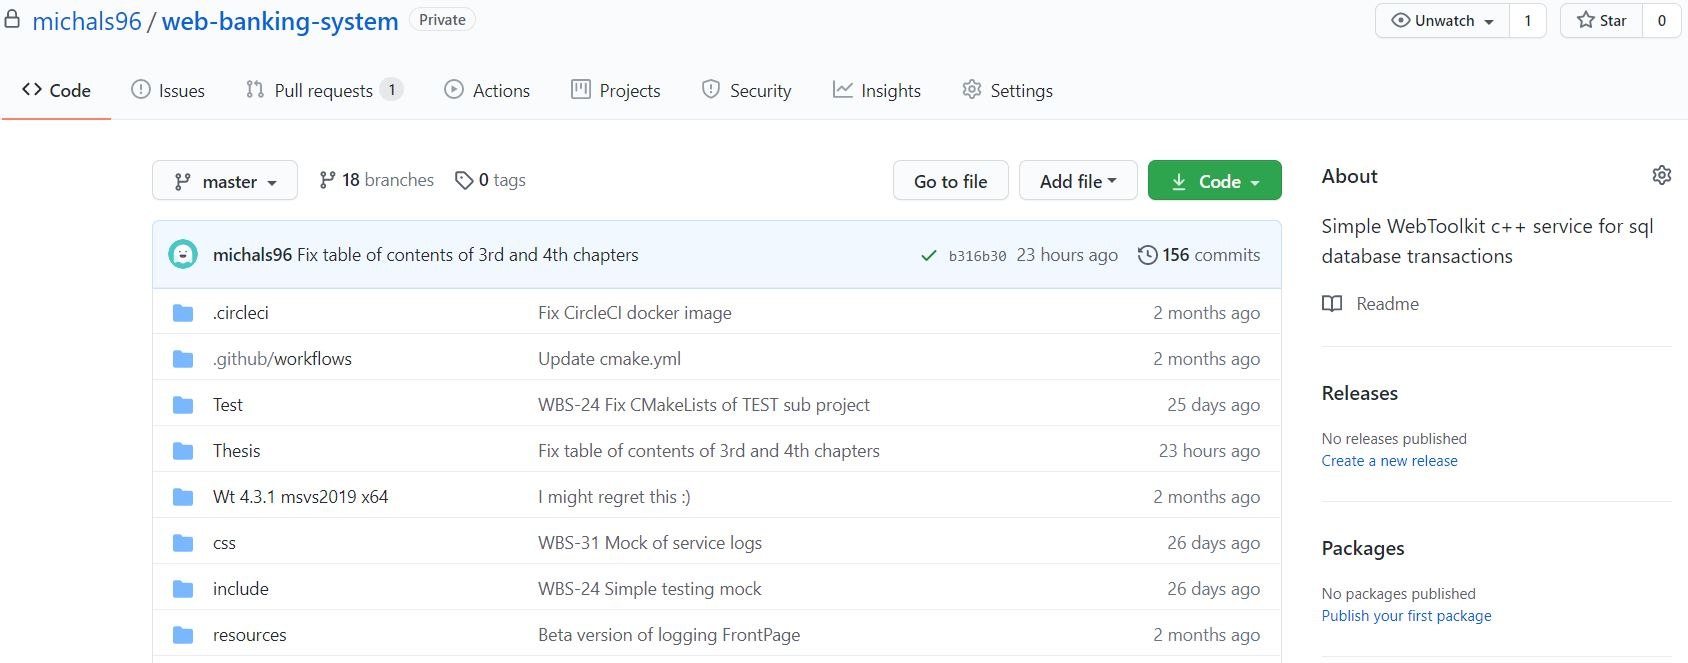
\includegraphics[width=1.0\textwidth]{repo}
    \caption{Web banking application github repository.~\cite{repo}}
\end{figure} 

\begin{figure}[H]
  \centering
    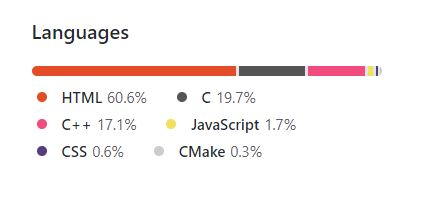
\includegraphics[width=0.7\textwidth]{languages}
    \caption{Languages statistics on Web banking application repository. The majority of is HTML code, because of the static resoruces of WebToolkit library, which handle HTML.~\cite{repo}}
\end{figure} 
    
\begin{figure}[H]
  \centering
    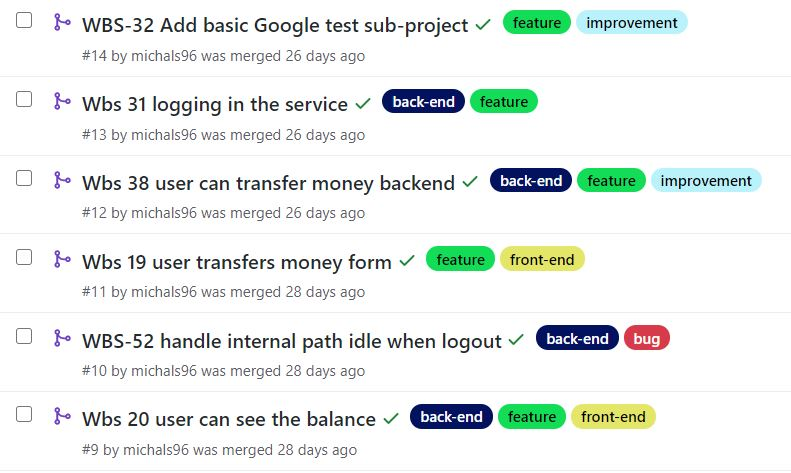
\includegraphics[width=0.7\textwidth]{pullrequests}
    \caption{A small batch of a few pull requests done during the implementation.~\cite{repo}}
\end{figure} 
    
A pull request itself is a github feature which allows programmers to do a review of a code that has been developed during a certain amount of time and is now to be ready to be merged to the main branch of the repository, which is usually the branch that is frequently being built and released to the client. This process performs a quality gate to the code and also increases readability of the changes introduced to the product. Figure 3.5 shows a few pull requests that were put out during the development. Each one of the pull requests has its unique name, id and can be also labeled by fancy labels (like feature, bug, improvement, back-end and others) which can be modified by repository owners. Before merging, the product is being built with the upcoming changes, which is another quality gate. If the built is successful and the reviewers approved the code - a programmer is allowed to merge the code and close the pull request. Another interesting thing is that every pull request or commit may be pre-tagged with a \textbf{WBS-number}, which stands for "WebBankingApplication-number of the story" and is thoroughly explained in the next section of this chapter. 
}
\section{Proprietary issue tracking}
{
\tab Another tool that came in really handy during development is proprietary issue tracking. It is a system which reflects changes introduced to the project and ultimately allows to track and manage the progress. 
}
\subsection{JIRA Software}
{
\tab An issue tracking system which was used in the project is JIRA Software. With its graphic user interface it can provide a projects board  which reflects Agile framework chosen in a development process and later on it could impact on the way of presenting issues work flow in a different way. Agile framework is a set of organization patterns and work flow patterns that are followed in order to improve to development process. In the project we could group issues by those that are meant to be done, those that are being currently developed and those that are already done.

\bigskip
\begin{figure}[H]
  \centering
    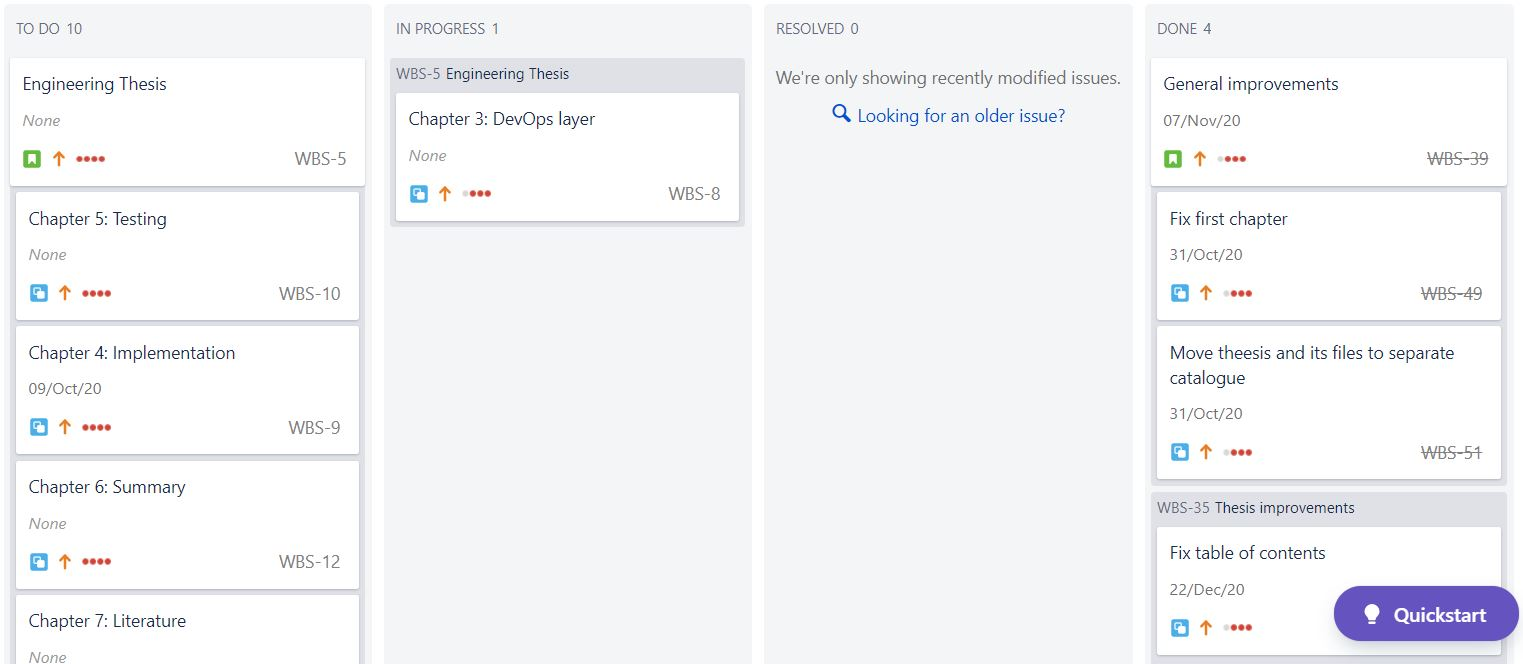
\includegraphics[width=1.0\textwidth]{kanban}
    \caption{JIRA Kanban board used during projects development.~\cite{jiraboard}}
\end{figure} 
    
\bigskip Kanban board is a board that reflects another work flow, where issues are reported and resolved as development goes, without working in a frequent time rate like in Scrum where developers could work for example in two week sprint methodology. Nevertheless, before starting programming Web banking application, the whole development process needed to be thought through and planned well. After planning, issues were created and added to the board. With creating every part of the project there was an issue that reflected actual state of the task that is being worked on. Swift GUI of JIRA Software allows to easily do drag-and-drop, starting with issues in "To Do", ending up with issues in "Done" table.
    
\bigskip
In this project issues were group by
\begin{itemize}
	\item engineering thesis issues (mostly chapters),
	\item theesis improvements,
	\item application improvements,
	\item general improvements,
	\item and code of the application.
\end{itemize}
	
JIRA Software allows developers to connect project issue tracking with its repository and during this development it was no different - github repository was connectet with JIRA. What it does is it detects branches and pull requests by id in commits (mentioned in previous section) that are binded to the given story or issue. It improves managing the project work flow by allowing to track the code that was merged to accomplish particular issues. All a developer needs to do is to remember to include repository acronym in commit message as a tag. In this case it was "WBS". There is a possibility to set on a repository that commits without project tag cannot be push onto remote repository, which is guarding the quality of branching.

\begin{figure}[H]
  \centering
    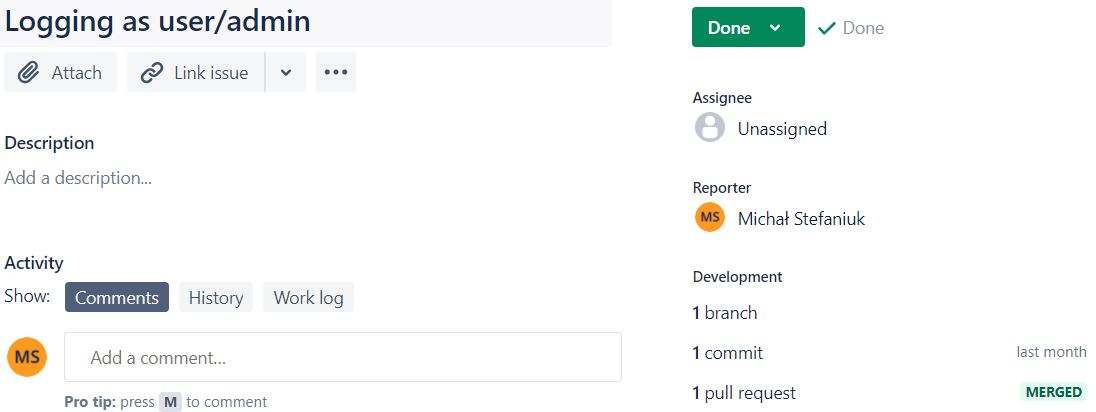
\includegraphics[width=1.0\textwidth]{issue}
    \caption{Adding project tags to commit messages on a repository that is connected with jira board detects the code created to resolve particular story ("Development" panel on the right).~\cite{jiraboard}}
\end{figure} 
    
\begin{figure}[H]
  \centering
    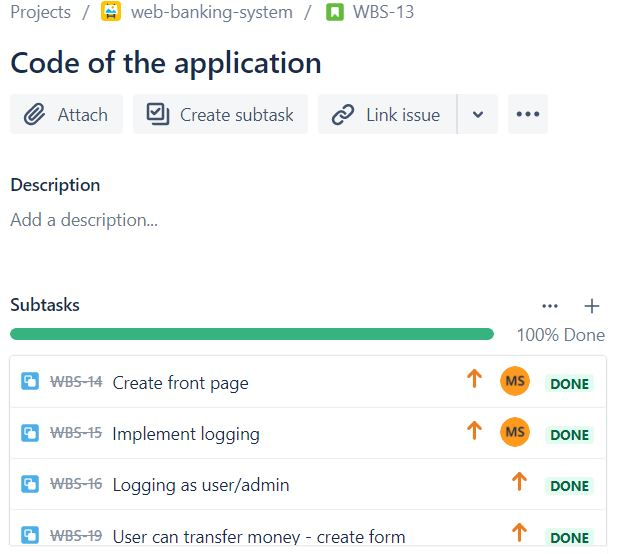
\includegraphics[width=0.5\textwidth]{applicationstory}
    \caption{Example story with subtasks.~\cite{jiraboard}}
\end{figure}
    
\bigskip
Apart from project board JIRA provides many other features like for example simple reports, that are usually presented on graphs that are available by a single click.      
Estimating due dates and development duration is also a very important part of tracking issues. However in this project only due dates were estimated  as Kanban framework does not expect estimating the duration for each issue. All in all, the project was planned for 5 stories, with around 38 subtasks. Those which were not chosen to be developed and were not completed were archived in backlog section of the board.

\begin{figure}[H]
  \centering
    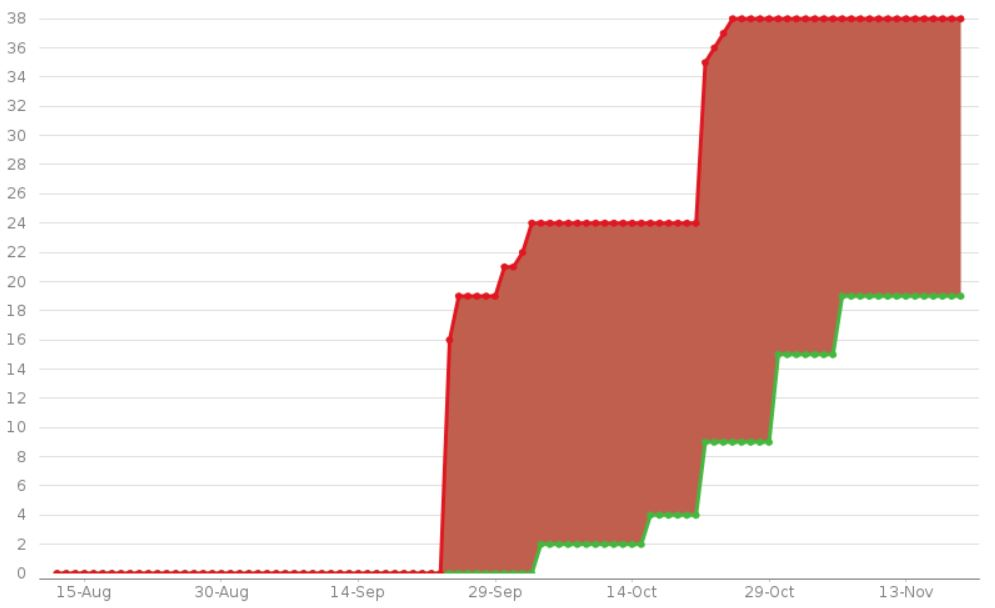
\includegraphics[width=1.0\textwidth]{chart1}
    \caption{ This chart shows the number of issues created vs. the number of issues resolved in the last 100 days.~\cite{jiraboard}}
\end{figure}
    
}

\section{Automation server and regression testing}
{
\tab Software development should not be done without assuring that the quality of the product is there. Among many quality gates like code review or unit testing there is also another one equally important - regression testing. It is being run on an automation server, which usually is another software that helps to automate the building process by configuring tasks, so called "jobs". It can also be used as a documentation generator. It is a common practice to run regression testing as well, which are nothing but a functional or non-functional test scenarios that ensure that the code that is about to be merged won't have a negative impact on the product. In a nutshell - regression testing will also verify if the software that is being developed works at all the time, considering that the regression tests might be run not only when a programmer tries to modify the code, but also when the code is merged. As a matter fact, there are many testing approaches when it comes to regression. For instance - the tests that are causing the highest traffic on the automation server might be run over night or during the weekend when developers are not working. It is a very powerful tool which can have a major impact on the quality of the development.

\bigskip During implementing web banking application, an automation server was set up, which was connected to the repository where the code was stored. This server was also set up on a GitHub, as a part of the repository. Anyone who owns a repository in this service can set such server by himself. All it is required is to go into actions section of repository settings and choosing a specific workflow that we would like to set up. Everything can be done in a few minutes and it does not require any specific knowledge. It is provided by GitHub for free with certain limitations - 20,000 minutes a month of testing is available. Anything more than this requires subscribing to the paid edition.  

\bigskip With each pull request, automation server took changes that were about to be merged. Then the server has been building specific branch and if the build was successful, it went to another job which was running the regression test. If every job has passed successfully, then the developer was allowed to merged the code - that is assuming that the code review was already done.

\begin{figure}[H]
  \centering
    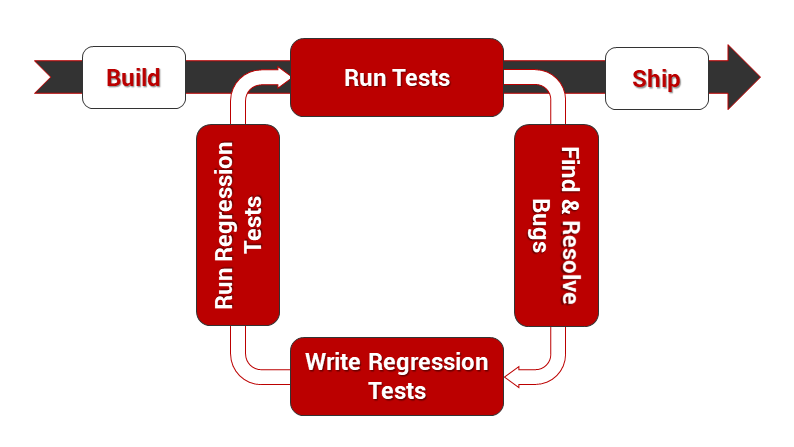
\includegraphics[width=1.0\textwidth]{regression}
    \caption{Regression testing.~\cite{reg}}
\end{figure}

}
\subsection{GitHub CMake}
{
\tab The automation server that was used in a project is GitHub CMake. It is basically provided by github and it's free. All it takes is to define a CMake file that describes building dependencies for the project. Automation server will fetch it and build the application on it's remote machine with Linux's Ubuntu distribution. From this point, when the application is remotely build, regression testing might be started.

\begin{figure}[H]
  \centering
    
\includegraphics[width=0.8\textwidth]{checks}
    \caption{When a pull request is created, automation server triggers and verifies incoming changes by building the project and running testes.}
\end{figure}

\bigskip To be able to add a test case scenario, first it must be implemented. In web banking application ctest was used, which is just a part of CMake and as an executable it enables testing, adds tests, runs them and reports results.
    
\bigskip
\begin{lstlisting}[frame=single, basicstyle=\small, language=C++, caption={Example ctest file used in project. It is quite self-explanatory, if first input argument equals 0, the scenario prints 'SUCCESS' and exits with 0 status. Otherwise it prints 'FAIL' and exit with 1 status.}, captionpos=b, float]
#ifndef _WIN32
#include <stdio.h>
#include <stdlib.h>

int main(int argc, char** argv) {
    if (argc < 2) {
        printf("usage: test <argument>\n");
        printf("If <argument> is 0, print SUCCESS. Otherwise print FAIL.\n");
        exit(1);
    }

    if (atoi(argv[1]) == 0) {
        printf("SUCCESS\n");
        exit(0);
    }
    else {
        printf("FAIL\n");
        exit(1);
    }
}
#endif
\end{lstlisting}

\bigskip Having test implemented in place, a scenarios must be defined in CMake file, that will report the results. 
\bigskip
\begin{lstlisting}[frame=single, basicstyle=\small, language=C++, caption={Example CMakeLists file used to define scenarios. In first two lines source code file and executable are set. Then by callig add test a scenario is added with input arguments. In the next lines, set test properties will define expected behaviour.}, captionpos=b]
SET(CTEST_SRC {CTEST_SRC} ctest.cpp)
add_executable(test {CTEST_SRC})

add_test(usage_test test)
set_tests_properties(usage_test PROPERTIES WILL_FAIL TRUE)

add_test(success_test test 0)
set_tests_properties(success_test PROPERTIES PASS_REGULAR_EXPRESSION "SUCCESS")

add_test(fail_test test 1)
set_tests_properties(fail_test PROPERTIES WILL_FAIL TRUE)

add_test(fail_test_output test 1)
set_tests_properties(fail_test_output PROPERTIES PASS_REGULAR_EXPRESSION "FAIL")
\end{lstlisting}

\bigskip Including above CMakeLists file in the project will trigger running four test case scenarios with each regression run.

\begin{figure}[H]
  \centering
    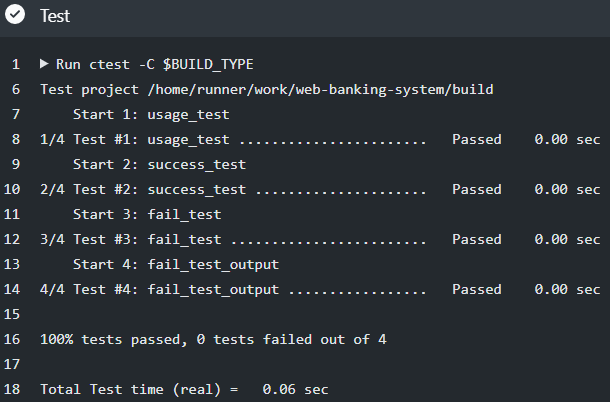
\includegraphics[width=0.8\textwidth]{testreg}
    \caption{Regression job responsible for running tests and verifying the results.}
\end{figure}
}
\subsubsection{Regression Docker file}
{
\tab Docker is a software that realizes the concept of virtualization at OS level. By composing a docker image, a developer is able to create precise programming environment in a container, in which it possible to run any desired application. It is a lighter way of virtualization, rather than setting up a virtual machine.      

\begin{figure}[H]
  \centering
    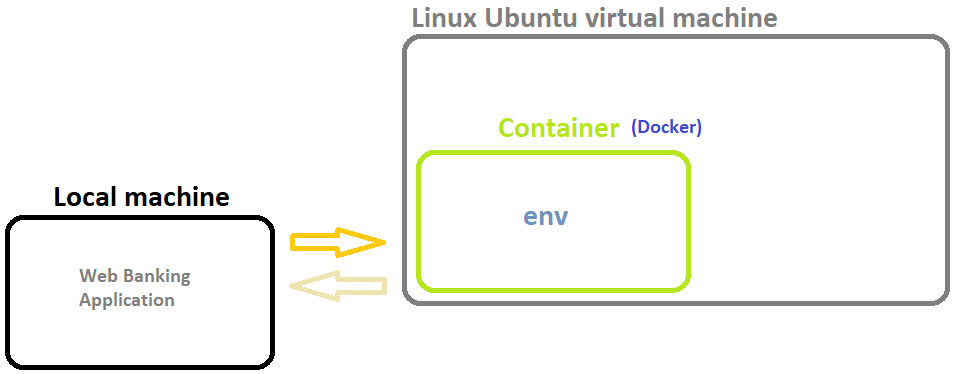
\includegraphics[width=0.8\textwidth]{scheme}
    \caption{Github CMake provides Linux virtual machine for the developers, where Docker container with a specific environment is set up.}
\end{figure} 
    
\bigskip 
To set up the machine responsible for automation one must place docker file all necessary dependencies. The jobs that has been set up are: 
    
\begin{labeling}{alligator}
\item [\textbf{Set up job}] Loads Ubuntu 18.04.5 LTS operating system, prepares workflow directory and all required actions.

\item [\textbf{Run actions/checkout@v2}] Fetches the repository, gets git version and authorizes user.

\item [\textbf{Get Boost libraries}] Downloads and installs Boost.

\item [\textbf{Create build environment}] Makes build directory for output files.

\item [\textbf{Configure CMake}] Identifies compilers.

\item [\textbf{Build}] Builds the project.

\item [\textbf{Test}] Runs regressions tests.

\item [\textbf{Post Run actions/checkout@v2}] Post job cleanup.

\item [\textbf{Complete job}] Cleaning up orphan processes.
\end{labeling} 
    
\begin{figure}[H]
  \centering
    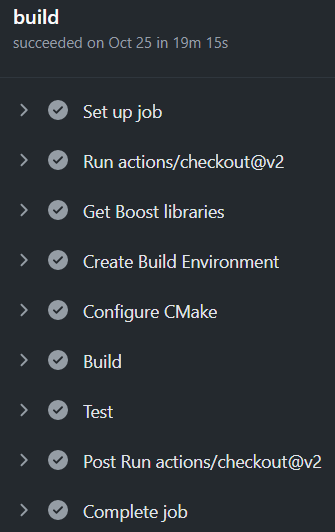
\includegraphics[width=0.4\textwidth]{jobs}
    \caption{Github CMake jobs.}
\end{figure}  

\begin{lstlisting}[frame=single, basicstyle=\small, language=C++, caption={cmake.yaml docker image used in project to set up automation server.}, captionpos=b, float]
name: CMake

on: [push]

env:
  BUILD_TYPE: Release

jobs:
  build:
    runs-on: ubuntu-latest

    steps:
    - uses: actions/checkout@v2
      
    - name: Get Boost libraries
      run: sudo apt-get install libboost-all-dev
      
    - name: Create Build Environment
      run: cmake -E make_directory ${{runner.workspace}}/build

    - name: Configure CMake
      shell: bash
      working-directory: ${{runner.workspace}}/build
      run: cmake $GITHUB_WORKSPACE -DCMAKE_BUILD_TYPE=$BUILD_TYPE

    - name: Build
      working-directory: ${{runner.workspace}}/build
      shell: bash
      run: cmake --build . --config $BUILD_TYPE

    - name: Test
      working-directory: ${{runner.workspace}}/build
      shell: bash
      run: ctest -C $BUILD_TYPE
\end{lstlisting}
}

\chapter{Implementation}

The Web Banking Application contains four major fields which will be described in further sections. Among those, there are:
  
\begin{itemize}
\setlength\itemsep{0em}
\item core class,
\item widgets,
\item session,
\item user entity,
\item and database.
\end{itemize}

\begin{figure}[H]
\centering
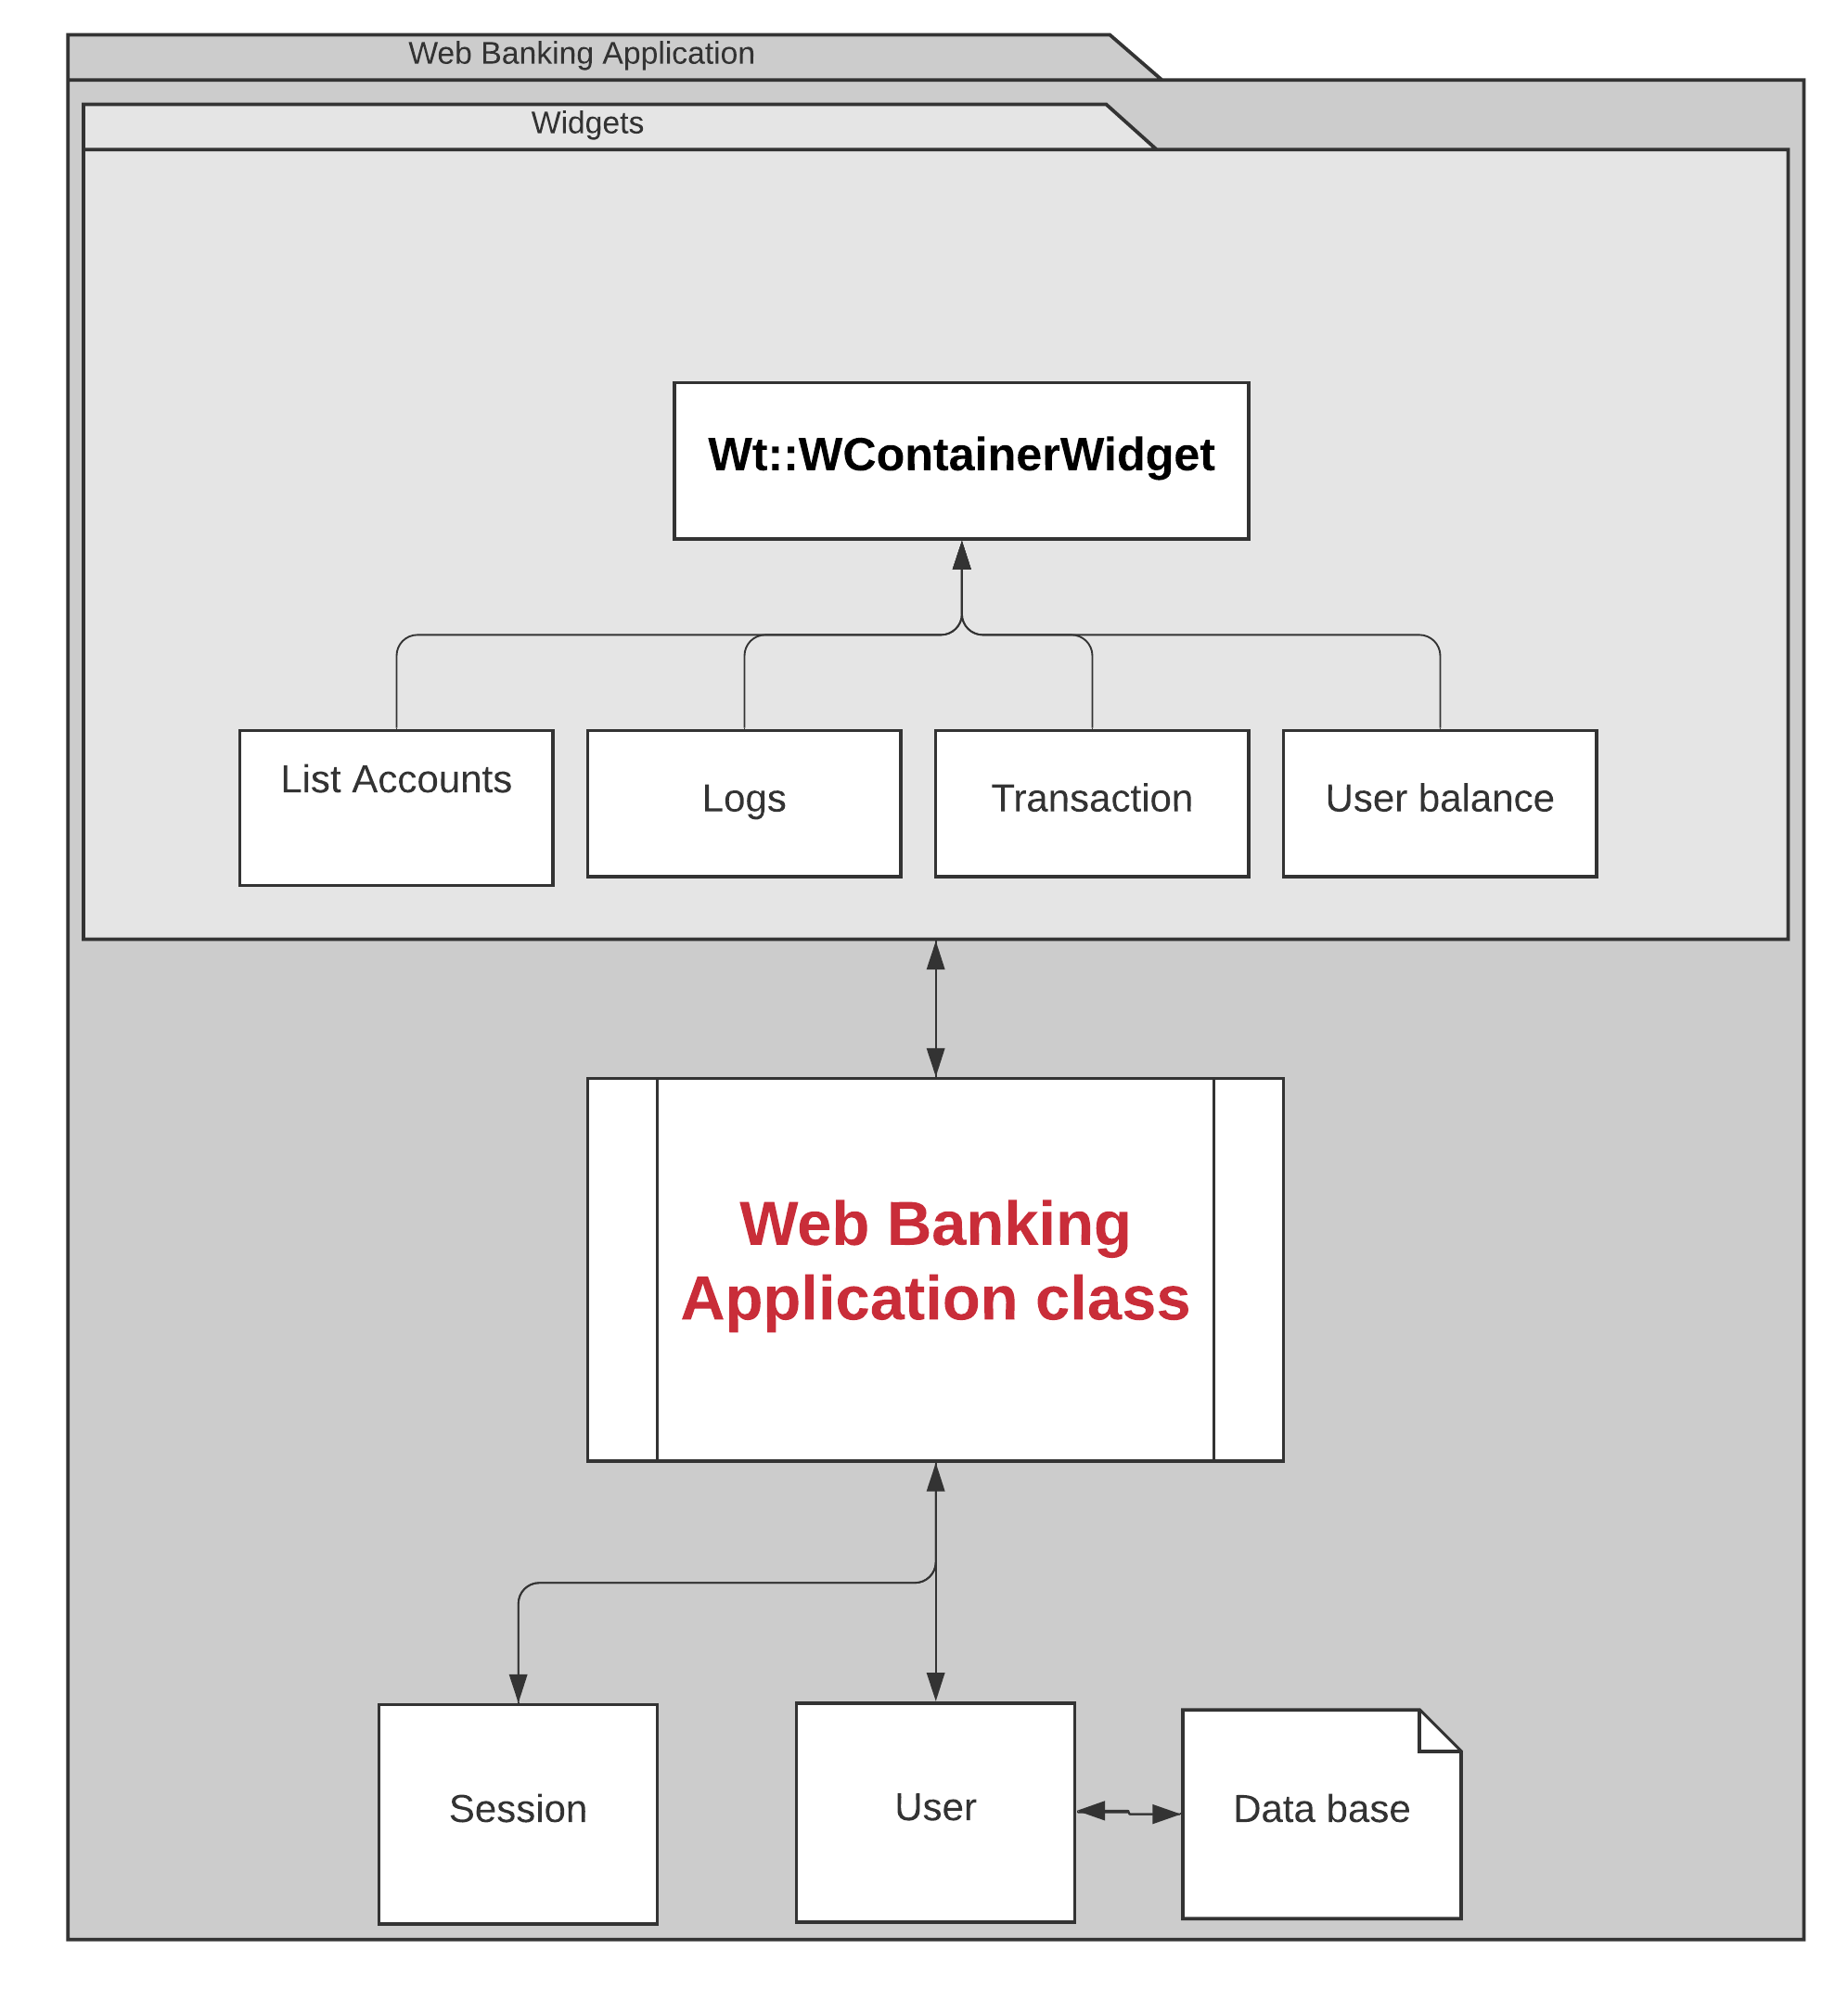
\includegraphics[width=0.7\textwidth]{uml2}
\caption{UML implementation diagram of the application.}
\end{figure}

\section{Web Banking core class}
{
The class represented in listing~\ref{lst:coreclass} is the main class that holds all necessary service functionalities and business logic.  
\bigskip
\begin{lstlisting}[frame=single,label={lst:coreclass}, basicstyle=\small, language=C++, caption={WebBankingApplication.h file. Most members are private because they are supposed only to be used in this class, apart from handleInternalPath() which could be used in other widgets that would want to impact the url path. The biggest disadvantage of current implementation is the class became really swell and in future it should be separated into two classes holding user and admin features individually. However the current solution is really simple, which is its biggest advantage. If a programmer would like to add a new page representing new feature, he should first create a new widget were rules of rendering content would be described. Then he should have add an object of this widget in this class and create a function which would clear current widget container and plug the new widget. This function would be called in handle internal path and it would be triggered upon URL change, which as we now would happen by clicking new WAnchor object. }, captionpos=b]
class WebBankingApplication : public Wt::WContainerWidget
{
public:
	WebBankingApplication();
	void handleInternalPath(const std::string& internalPath);
	
private:
	// Acts like a container for widgets
	WStackedWidget       *mainStack;
	// Widgets responsible for user and admin features
	UserBalanceWidget    *userBalance;
	ListAccountsWidget   *accounts;
	TransactionsWidget   *transactions;
	LogsWidget			 *logs;
	// Widgets that show box with links
	// for admin and user
	WContainerWidget     *userLinks;
	WContainerWidget	 *adminLinks;
	
	// WAchor is a link which
	// changes URL upon clicking
	WAnchor* balanceAnchor;
	WAnchor* transactionAnchor;
	WAnchor* listUsersAnchor;
	WAnchor* serviceLogsAnchor;
	
	Session session;
	
	// This function veryfies if user is logged in
	// and who is logged in. Regarding this information
	// it renders admin menu, user menu or login panel.
	void onAuthEvent();	
	
	// Those functions are reponsible for
	// plugging individual widgets
	void showUserBalance();
	void showAllAccounts();
	void showTransactionPanel();
	void showServiceLogs();
};
\end{lstlisting}

\bigskip
This class derives  from Wt::WContainerWidget class, which is built-in WebToolkit class that behaves like a container for widgets. In the application the logic is that widgets are created and depending on which one user wants to use, the application plugs in or plugs them out of the WebBankingClass container. In the constructor of this class the application creates a Session, which is a link between processes and connects with it. Then it creates Wt::WtStackedWidget object, which will hold widgets and plugs in logging page widget into it. At the end it connects with handleInternalPath signal and start processing the whole environment. 

\bigskip
Constatly calling handleInternalPath() function will put on a guardian, which will react to any changes in URL internal path. The logic inside of this function is whenever a path is changed, different widget will be plugged in the container, which ultimately will cause in rendering different content for the application user.

\bigskip
\begin{lstlisting}[frame=single, basicstyle=\small, language=C++, caption={handleInternalPath() function.}, captionpos=b]
void WebBankingApplication::handleInternalPath(const std::string& internalPath)
{
	if (session.login().loggedIn() && session.userName() != "admin") 
	{
		if (internalPath == "/balance")
		{

			showUserBalance();
		}
		else if (internalPath == "/transaction")
		{

			showTransactionPanel();
		}
		else
		{
			WApplication::instance()->setInternalPath("/", true);
		}
	}
	else if (session.login().loggedIn() && session.userName() == "admin")
	{
		if (internalPath == "/accounts")
		{
			showAllAccounts();
		}
		else if (internalPath == "/logs")
		{
			showServiceLogs();
		}
		else
		{
			WApplication::instance()->setInternalPath("/", true);
		}
	}
	else if (session.login().loggedIn() == false)
	{
		WApplication::instance()->setInternalPath("", true);
	}
}
};
\end{lstlisting}

\begin{figure}[H]
\centering
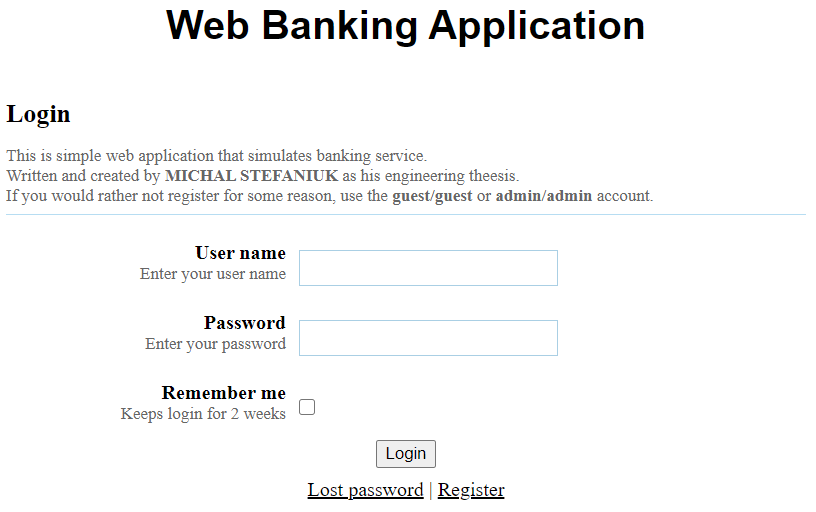
\includegraphics[width=1.0\textwidth]{logpage}
\caption{This is the page that renders to user when he turns the application on. Default logging widget is plugged in.}
\end{figure}  

Other members of this class are just widgets and methods responsible for plugging them-in, which is the topic of the next section.
}
\section{Widgets}
{
\section*{List accounts widget}
{

This widget renders one of admin functionalities. It is responsible for listing all users in the service with their balance. 

\begin{figure}[H]
\centering
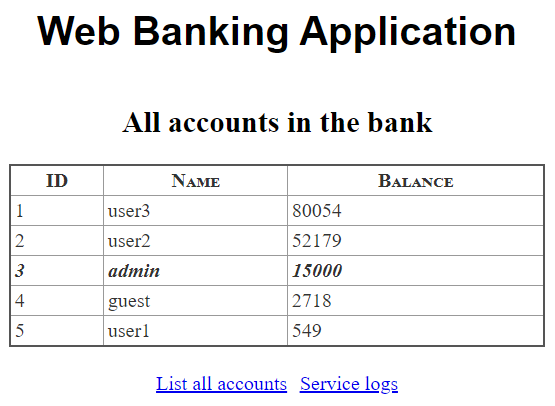
\includegraphics[width=0.7\textwidth]{listaccounts}
\caption{This is the page that renders to user when he logs as an admin and chooses to list all accounts.}
\end{figure}  

The code of this class is rather really simple. It derives from WContainerWidget and has only two methods. First one is constructor, which only initializes parent class and session. Second one is update() function which is responsible for composing the widget with table.

\bigskip
\begin{lstlisting}[frame=single, basicstyle=\small, language=C++, caption={ListAccountsWidget::update() function.}, captionpos=b]
void ListAccountsWidget::update()
{
    clear();

    this->addWidget(cpp14::make_unique<WText>
    ("<h2> All accounts in the bank </h2>"));

    std::vector<User> top = session_->getUsers();

    WTable* table = this->addWidget(cpp14::make_unique<WTable>());

    table->elementAt(0, 0)->addWidget(cpp14::make_unique<WText>("ID"));
    table->elementAt(0, 1)->addWidget(cpp14::make_unique<WText>("Name"));
    table->elementAt(0, 2)->addWidget(cpp14::make_unique<WText>("Balance"));
    table->setHeaderCount(1);

    for (auto& user : top) {
        int row = table->rowCount();

        table->elementAt(row, 0)->addWidget
        (cpp14::make_unique<WText>(user.id));
        
        table->elementAt(row, 1)->addWidget
        (cpp14::make_unique<WText>(user.name));
        
        table->elementAt(row, 2)->addWidget
        (cpp14::make_unique<WText>(asString(user.balance)));
    }
}
\end{lstlisting}

At the beginning of update() function in this widget, a list of users is fetched from the database by calling getUsers() and it is being assigned to the top vector. Then a very basic table is being constructed in a for loop regarding the information about users in top vector. When the iteration is finished, the widget is composed and rendered. Plugging the widget to the front page was already done in line 10, by callid addWidget() function on this object.
}

\section*{Logs widget}
{
This widget is responsible for rendering service logs from the transactions that has been conducted among certain accounts. It is a second and the last admin functionality.

\begin{figure}[H]
\centering
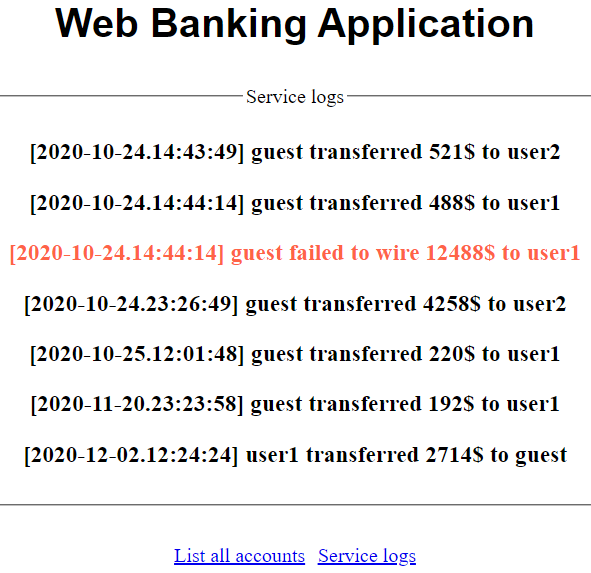
\includegraphics[width=0.7\textwidth]{servicelogs}
\caption{This is the page that renders to user when he logs as an admin and chooses to list all transactions.}
\end{figure}

\bigskip
The implementation is just the same as in every widget in this application. Derivation from WContainerWidget, constructor, update method for constructing the widget and a session member.

\bigskip
\begin{lstlisting}[frame=single, basicstyle=\small, language=C++, caption={LogsWidget::update() function.}, captionpos=b]
void LogsWidget::update()
{
	clear();

	auto groupBox = Wt::cpp14::make_unique<Wt::WGroupBox>("Service logs");
	groupBox->addStyleClass("centered-example");

	std::ifstream file("logs.txt");
	if (file.is_open()) {
		std::string line;
		while (std::getline(file, line)) {
			groupBox->addNew<Wt::WText>(line.c_str());
		}

		this->addWidget(std::move(groupBox));

		file.close();
	}
}
\end{lstlisting}

What is interesting about this widget is its construction in update() function. As in every widget, in the beginning all widgets from the page are removed by calling clear() function. Then, a group box is created, which is  another type of table that is built in and provided by default Web Toolkit library. Then, a file called logs.txt is being opened. It is a file that contains informations about transactions - when a transaction is made, logs are appended to this file. If it doesn't exist, no logs are rendered. As the file is loaded, it is iterated line by line. With each iteration a line with transaction information is added to the groupBox, which ultimately constructs the whole widget. Then it is added to the page. From the security point of view this is not the safest approach for storing and fetching any kind of service logs, especially as fragile ones as the ones from banking application. To increase security of this mechanism the logs could have been encrypted and decrypted upon loading. Better yet, they could have been stored as an object in a database, which could have been stored in a various places limiting an access to those logs, by for instance authorizing potential clients. 
}

\section*{Transaction widget}
{
This widget is the first one that is provided by the service to the user without admin permissions. It is a panel, that allows user to actually conduct a simple transaction which is wiring money.

\begin{figure}[H]
\centering
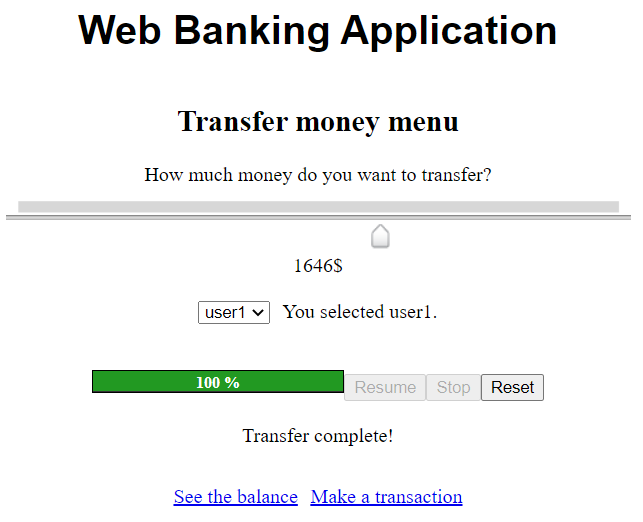
\includegraphics[width=0.7\textwidth]{wire}
\caption{This is the page that renders to user without admin permissions when chooses to make a transaction.}
\end{figure}

The wiring menu is rather simple. At the very top there is a slider where user can point out how much money he wants to wire. It is a nice show-how of the Web Toolkit library. By using built in slider widget it is possible to create an animation on the page without writing single javascript line of code. Then a user can choose to who he wants to wire the money. The last box is where a user can start a transaction and while it's being processed, he can stop it or reset the whole menu. When a transfer is completed, a notification appears.

\bigskip 
Although TransactionsWidget implementation is rather classic as it is for every widget in this application, there are a few additions to this particular widget. There is member log() function that is being called upon every transaction and it appends to logs.txt file information about the transfer that has just been made. The update function has a lot of boilerplate code which is responsible for the built in widgets (like the slider), so instead focusing on the whole update() function let's just take a look about the most important part which is the lambda responsible for handling the wiring itself.

\bigskip
\begin{lstlisting}[frame=single, basicstyle=\small, language=C++, caption={Part of TransactionWidget::update() function.}, captionpos=b]
intervalTimer->timeout().connect([=] {
	bar->setValue(bar->value() + 1);
	if (bar->value() == 10) {
		session_->addToBalance(transactionUsers[cb->currentIndex()].name,
		session_->userName(), slider->value());
		
		log(transactionUsers[cb->currentIndex()].name, 
		session_->userName(), slider->value(), true);
		
		stopButton->clicked().emit(Wt::WMouseEvent());
		startButton->disable();
		
		this->addWidget(cpp14::make_unique<WBreak>());
		this->addWidget(std::move(cpp14::make_unique<WText>("Transfer 
		complete!")));
	}
});
\end{lstlisting}

In the beginning of this lambda function, we connect a timeout(), which is a signal emmited after the timer times out, to the intervalTimer which generates those signals when a start() function is being called. So basically whenever user presses "Start" button to wire money, this lambda is being called. First we increment the value of the slider by one just to get the animation going. It's just a visual efect, but it also gives user a chance to stop the transaction. When the bar slider has reached an end, addToBalance() function is called, which finds source and target user and updates their balances by adding or subtracting money. Then a log() function is called - at this point we know what it's responsible for. The rest of the logic is just disabling start button, clicking stop button and printing "Transfer complete!" notification.
}

\section*{User balance widget}
{
This is the second and the last widget provided by the service to the user without admin permissions. It is a very basic one, which prints the information about current user's balance.

\begin{figure}[H]
\centering
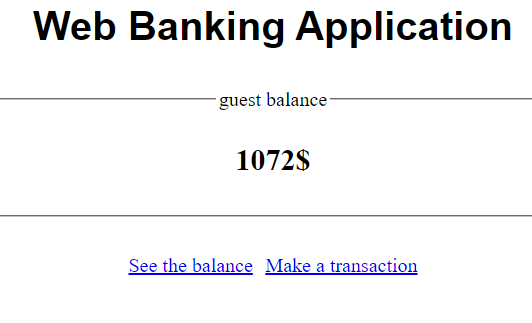
\includegraphics[width=0.7\textwidth]{balance}
\caption{This is the page that renders to user without admin permissions when he chooses to see the balance.}
\end{figure}

The update() function for this widget is very transparent. What it does is it just fetches users from the database and the user that is just logged. Then it compares logged user to the one in a database and if it finds the user, it fetches his balance. Lastly, the balance is added to the simple groupBox, which is later added to the widget container and that is how user balance widget is being composed.

\bigskip
\begin{lstlisting}[frame=single, basicstyle=\small, language=C++, caption={UserBalanceWidget::update() function.}, captionpos=b]
void UserBalanceWidget::update()
{
	clear();

	int userBalance = 0;

	std::string userName = session_->userName();
	std::vector<User> top = session_->topUsers();

	for (auto& user : top) {
		if (user.name == userName) {
			userBalance = user.balance;
		}
	}

	auto groupBox = Wt::cpp14::make_unique<Wt::WGroupBox>(userName + " balance");
	groupBox->addStyleClass("centered-example");

	std::string userBalanceStr = std::to_string(userBalance);
	groupBox->addNew<Wt::WText>("<h2>" + userBalanceStr + "$</h2>");
	this->addWidget(std::move(groupBox));
}
\end{lstlisting}
}

}
\section{Session}
{
Knowing that HTTP is a stateless protocol we have to point out one very important thing. WWW server will process each transaction independently, without looking for any relations to other transactions commited by the user. This means that it is almost impossible for an application to track all systems of authorization that require to track every user activity within the application. For example - if we log in the service at the logging page, how does the service know at the next page that we are still logged in? The answer is it doesn't. To be more precise - it doesn't until it's provided with lasting entity carrying information, that could be passed between components. The answer to this challenge is session. It is a class that is equipped with business logic that allows it to carry valuable information from the service point of view and may be passed between components. It can be simulated when we use dynamic language like C++. In many languages it is a common practice to implement session, like for instance when coding a server-side of the application in PHP. 

\bigskip
\begin{lstlisting}[frame=single, basicstyle=\small, language=C++, caption={Session.h file.}, captionpos=b]
typedef Auth::Dbo::UserDatabase<AuthInfo> UserDatabase;

class Session
{
public:
	static void configureAuth();

	Session();
	~Session();

	Auth::AbstractUserDatabase& users();
	Wt::Auth::Login& login();
	std::vector<User> topUsers(int limit);
	std::string userName() const;
	int findId();
	void addToBalance(std::string tgtName, std::string srcName, int amount);

	static const Auth::AuthService& auth();
	static const Auth::AbstractPasswordService& passwordAuth();
	static const std::vector<const Auth::OAuthService*>& oAuth();

private:
	mutable Dbo::Session session_;
	Wt::Auth::Login login_;
	std::unique_ptr<UserDatabase> users_;
	Dbo::ptr<User> user() const;
};
\end{lstlisting}

Most of the methods are just getters to the private fields which are mostly WebToolkit built-in type variables. They are already provided with many valuable methods like for instance querying the database objects directly. The most important part of session logic are topUsers() and addToBalance() methods and those are the ones that we will focus on. 

\bigskip
When it comes to topUsers() method, it is used in every method that tries to modify the state of the database or in method that wants to fetch information about the users in the service.

\bigskip
\begin{lstlisting}[frame=single, basicstyle=\small, language=C++, caption={Session::topUsers() method.}, captionpos=b]
std::vector<User> Session::topUsers(int limit)
{
	dbo::Transaction transaction(session_);

	Users top = session_.find<User>().orderBy("balance desc").limit(limit);

	std::vector<User> result;
	
	for (Users::const_iterator i = top.begin(); i != top.end(); ++i) 
	{
		dbo::ptr<User> user = *i;
		result.push_back(*user);

		result.back().name = user->name;
	}

	transaction.commit();

	return result;
}
\end{lstlisting}

\bigskip
In the very beginning a transaction object is created using current session. Then all users are being assigned to top variable. This is the place in code where idea behind session concept clarifies. To fetch all users from database, find() method is being called on current session with chain of orderBy and limit methods. This will trigger a native query on a sqlite application database, which is actually visible in an application admin console. Second part of this method just iterates through User object pushing back each user to the vector which is being returned as a result. Of course, before returning this vector, a transaction must be commited.

\begin{figure}[H]
\centering
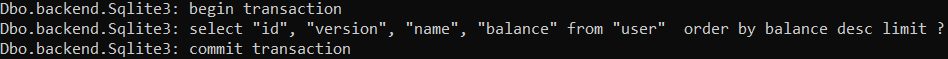
\includegraphics[width=1.0\textwidth]{transaction}
\caption{This is a really classic model for a database transaction. First a transaction is being made, then it's being created and when it's done, it is commited.}
\end{figure}

\bigskip
The second equally important method is addToBalance(). As mentioned before, it is quite self-explanatory. It's job is to find two users, the one that wants to wire some money and the one that the money will be transferred to. Next thing that this functions does, is it updates balances of both subjects of this transaction. The whole logic is completed by commiting such transaction, which obviously needs to be opened at the very beginning.

\bigskip
\begin{lstlisting}[frame=single, basicstyle=\small, language=C++, caption={Session::addToBalance() method.}, captionpos=b]
void Session::addToBalance(std::string tgtName, std::string srcName, int amount)
{
	dbo::Transaction transaction(session_);

	dbo::ptr<User> targetUser = 
		session_.find<User>().where("name = ?").bind(tgtName);

	targetUser.modify()->balance += amount;

	dbo::ptr<User> srcUser = 
		session_.find<User>().where("name = ?").bind(srcName);

	srcUser.modify()->balance -= amount;

	transaction.commit();
}
\end{lstlisting}

}
\section{User entity}
{
\tab User class is probably the most important class in Web Banking Application. It is a class that defines a structure of an user object that is being mapped to a database object. Later on, all operations rely on this content like for instance logging to the service or making transactions which is a core of the banking application.

\bigskip
\begin{lstlisting}[frame=single, basicstyle=\small, language=C++, caption={User class.}, captionpos=b]
class User;
typedef Wt::Auth::Dbo::AuthInfo<User> AuthInfo;
typedef dbo::collection< dbo::ptr<User> > Users;

class User
{
public:
	User();
    std::string name;
    int balance;
    dbo::collection<dbo::ptr<AuthInfo>> authInfos;

    template<class Action>
    void persist(Action& a)
    {
        dbo::field(a, name, "name");
        dbo::field(a, balance, "balance");
        dbo::hasMany(a, authInfos, dbo::ManyToOne, "user");
    }
};

DBO_EXTERN_TEMPLATES(User);
\end{lstlisting}
}

What is really interesting about this class is the way Web Toolkit transforms this class into the database object. To achieve this, it uses ORM operation. It stands for Object-Relational Mapping and it is a way of mapping an objective architecture of a single system to the database that has relational character. Such implementation is a common approach for applications that are implemented in an objective language using objective pattern. In this class there is only one persist() method defined. In this member function we define how Web Toolkit should map class member variables to database fields, so whenever an User object is created in code, Web Toolkit already knows how to put it into the database, if necessary. Other than that there are no methods whatsoever and the constructor is default. The class itself is rather really simple, there are three fields. Name, balance and authInfos for authentication upon logging. It is a built-in functionality provided by Web Toolkit. Let's jump into an example code which will get us closer to the idea behind using this class with object relational mapping.

\bigskip
\begin{lstlisting}[frame=single, basicstyle=\small, language=C++, caption={Example usage of object-relational mapping on User class. This logic happens in constructor of Session class, which is called upon turning the application on.}, captionpos=b]
	auto sqlite3 = cpp14::make_unique<Dbo::backend::Sqlite3>
	(WApplication::instance()->appRoot() + "WebBankingUserDatabase.db");

	sqlite3->setProperty("show-queries", "true");

	session_.setConnection(std::move(sqlite3));
	session_.mapClass<User>("user");
	session_.mapClass<AuthInfo>("auth_info");
	session_.mapClass<AuthInfo::AuthIdentityType>("auth_identity");
	session_.mapClass<AuthInfo::AuthTokenType>("auth_token");
	
	dbo::Transaction transaction(session_);
	try {
		session_.createTables();
	
		// Creating and inserting Auth Users
		Auth::User guestUser = users_->registerNew();
		guestUser.addIdentity(Auth::Identity::LoginName, "guest");
		myPasswordService.updatePassword(guestUser, "guest");
		
		/*
		Creating other auth users
		...
		*/
		
		// Creating reflection of Auth Users used in transactions
		std::unique_ptr<User> userGuest{ new User() };
		userGuest->name = "guest";
		userGuest->balance = 10000;
		dbo::ptr<User> userPtr = session_.add(std::move(userGuest));
		
		/*
		Creating other reflection users
		...
		*/
		
		log("info") << "Database created";
	}
	catch (...) {
		log("info") << "Using existing database";
	}

	transaction.commit();
		
\end{lstlisting}
	
\bigskip
At the very beginning sqlite database object is created. Then all necessary properties are set, including connecting current session with this database and setting mapping properties to user and authentication model. Then, as usually, a transaction is created and later on in a try block it is executed. At the beginning of try block createTables() function is being called on session object. If WebBankingUserDatabase.db already exists it will throw an exception which is then catched. This will cause in using already existing database. Otherwise try block will go further where new users are created and added to the database. Each user has to have two identities, first one for authentication purposes with login and password. Second one for business logic, which is a "reflection" of authentication user. 


\section{Database}
The database that was chosen for this application was sqlite3 data base. It is implemented in C language and it supports basic SQL language queries. The reason behind choosing sqlite is because it is natively supported by Web Toolkit and it's very light and simple. In the data base used in project we have three tables.

\subsection*{Authentication identity}
{
This table contains one of two reflections of users in the service. Those are actually the ones used for authentication during logging into the service. The most valuable information that this table carries is identity of the user auth info id which later on creates one-to-one relation with Authentication information table.

\begin{figure}[H]
\centering
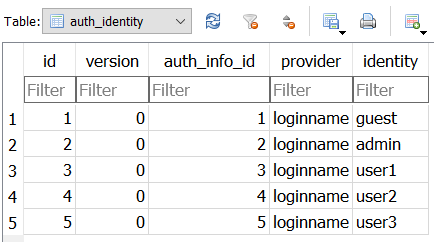
\includegraphics[width=0.7\textwidth]{auth_identity}
\caption{Authentication identity table.}
\end{figure}

}
\subsection*{Authentication information}
{
This table in realtion with Authentication identity creates a whole piece of record that is used to authenticate any user. It stores valuable and fragile information like password. Because of this fact, the password is encrypted with bcrypt method. In the database there is a password salt and password hash column - with those information it is possible to decrypt each password, but for the sake of security such information should not be stored in a plain text. There is also a table named "failed login attempts" which will increment with every failed login attempt an user makes.

\begin{figure}[H]
\centering
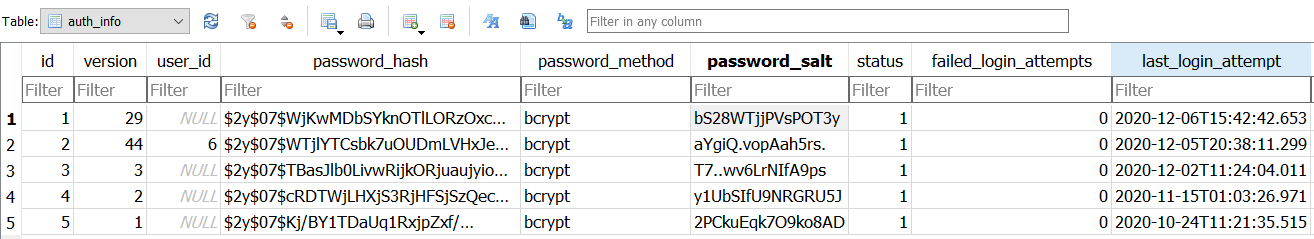
\includegraphics[width=1.0\textwidth]{auth_info}
\caption{Authentication information table.}
\end{figure}

}

\subsection*{User}
{
User table is the second one containing information about the users in the table, but this one is actually the one that is object-relational mapped from the code to the database object. Records from this table are also the ones used for transactions and other Web Banking Application features different then logging and authentication. It stores information about users name, balance and version, which actually shows an amount of changes that has been made to each record. For example if a guest's version is 17, it means that it was involved in 17 transactions.

\begin{figure}[H]
\centering
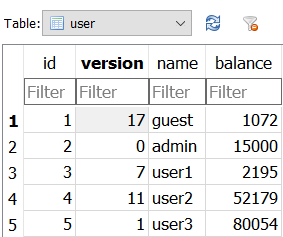
\includegraphics[width=0.6\textwidth]{user}
\caption{User table.}
\end{figure}
}
\chapter{Summary}
{

\tab The topic of this thesis was to create a web application that would simulate a banking service, which would allow to use software engineering tools during development. The finished application is a program that can be run by anyone and it realizes all the initial assumptions that were made at the beginning. During the implementation there were three tools established to enhance the development - GitHub repository, GitHub regression server and JIRA issue tracking tool. The GitHub version control system was extremely helpful especially when something needed to be debugged and fixed. Tracking changes in the project may have a huge impact on the development. JIRA software also helped a lot in tracking the actual state of the process of not only implementing the application, but also in writing this thesis. The regression testing came out to be more like a proof of concept, rather than an important quality gate. 

\bigskip
The biggest obstacle that was overcome during this development was lack of knowledge about Web Toolkit coding standards. This library introduces specific type of logic that may occur a bit unorthodox to many C++ developers. Another thing which came out to be troubling is rather small community behind Web Toolkit. Programming is many things, but one is for sure - there is no point in solving problems that were already solved (at least other than educational). While implementing this application almost every problem that came up had to be solved individually with no support from the programming forums whatsoever. This was actually really time consuming. 

\bigskip
The final application is quite flexible. From this point it could have been enhanced with many user features like for instance taking loans, banning users, setting transaction limits, creating sub accounts or even investing money. All it would take is making more widgets corresponding to each functionality. A front end layer could have been improved too with many fancy sliders, forms or widgets. When it comes to user interface - sky would be the limit.

\bigskip
It is a fact - one can actually implement a web application using C++ and although it is possible, it is not the most efficient way to go for when choosing technology stack. The standard technologies used for web development are javascript and html with css and it's because they are natively supported and easily interpreted by most web browsers. During the development it came clear that C++ library like Web Toolkit can only act as a wrapper for such technologies and it causes a lot of tricky riddles when it comes to debugging such code. Nevertheless, as a developer gets familiar with Web Toolkit concepts, the development rapidly speeds up and indeed, it could be used for creating simple single page web applications.

}
\begin{thebibliography}{9}
\bibitem{cmakeintroduction}
  Introduction to CMake,
  \emph{http://derekmolloy.ie/hello-world-introductions-to-cmake}.
  
\bibitem{singlepageapplications}
  Single Page Applications,
  \emph{https://www.excellentwebworld.com/what-is-a-single-page-application}.
  
\bibitem{wtlogo}
  WT Logo and Features,
  \emph{https://www.webtoolkit.eu/wt/features}.

\bibitem{authmodule}
  Introduction to Wt::Auth,
  \emph{https://www.webtoolkit.eu/wt/doc/tutorial/auth.html}.
  
\bibitem{helloworldapp}
  Wt Hello World Application,
  \emph{https://www.webtoolkit.eu/wt/doc/tutorial/wt.html}.

\bibitem{widgetsgallery}
  Wt Widgets Gallery,
  \emph{https://www.webtoolkit.eu/widgets/forms/}.
  
\bibitem{facebook}
  Facebook,
  \emph{https://www.facebook.com}.
  
\bibitem{airbnb}
  airbnb,
  \emph{https://www.airbnb.com}.
  
\bibitem{twitter}
  Twitter,
  \emph{https://www.twitter.com}.
  
\bibitem{paypal}
  payPal,
  \emph{https://www.paypal.com}.
  
\bibitem{gmail}
  gmail,
  \emph{https://www.gmail.com}.
  
\bibitem{netflix}
  Netflix,
  \emph{https://www.netflix.com}.

\bibitem{javascript}
  JavaScript,
  \emph{https://www.javascript.com/}.
  
\bibitem{typescript}
  TypeScript,
  \emph{https://www.typescriptlang.org/}.
  
\bibitem{html}
  HTML,
  \emph{https://www.w3schools.com/html/}.
  
\bibitem{css}
  CSS,
  \emph{https://www.w3schools.com/css/}.
 
\bibitem{java}
  Java,
  \emph{https://www.java.com/pl/}.
  
\bibitem{python}
  Python,
  \emph{https://www.python.org/}.
  
\bibitem{php}
  PHP,
  \emph{https://www.php.net/}.
  
\bibitem{html5}
  HTML5,
  \emph{https://developer.mozilla.org/pl/docs/HTML/HTML5}.
  
\bibitem{html4}
  HTML4,
  \emph{https://www.w3.org/TR/html5-diff/}.
  
\bibitem{lambda}
  C++11 lambda expressions,
  \emph{https://en.cppreference.com/w/cpp/language/lambda}.
  
\bibitem{opengl}
  OpenGL,
  \emph{https://www.opengl.org/}.
  
\bibitem{svg}
  HTML5 SVG,
  \emph{https://css-tricks.com/using-svg/}.

\bibitem{devops}
  devOps logo,
  \emph{https://www.netsparker.com/devops-security-tools/}.
  
\bibitem{git}
  Git workflow,
  \emph{https://panizkomputerem.pl/czym-jest-git/}.
  
\bibitem{repo}
  Applications github repository,
  \emph{https://github.com/michals96/web-banking-system}.   

\bibitem{jiraboard}
  JIRA board,
  \emph{https://www.atlassian.com/pl/software/jira}.   
  
\bibitem{reg}
  Regression testing,
  \emph{https://www.maveryx.com/automated-regression/?cn-reloaded=1}. 
\end{thebibliography}

\textbf{Additional materials} \begin{itemize}
	\item LaTeX wikibooks \newline \textit{https://en.wikibooks.org/wiki/LaTeX}

\end{itemize}

\linespread{1.3}
\selectfont

\end{document}